\PassOptionsToPackage{hidelinks}{hyperref}

\documentclass[jou,12pt,floatsintext]{apa7} % man doc stu jou


% 语言和字体设置
\usepackage[american]{babel}
\usepackage{ctex}
\usepackage{xeCJK}
\setCJKmainfont{Songti SC Regular} % 设置中文主字体为 STSong,字间距增加
\setmainfont{Times New Roman} % 设置英文字体

\setlength\parindent{2em}

% 参考文献设置
\usepackage{csquotes}
\usepackage[style=apa,sortcites=true,sorting=nyt,backend=biber]{biblatex}
\DeclareLanguageMapping{american}{american-apa}
\addbibresource{bibliography.bib}

%绘图用
\usepackage{caption}
\usepackage{graphicx}
\usepackage{float} 
\usepackage{subcaption}
\usepackage{stfloats}
% \usepackage{subfigure}





% Title page stuff _____________________
\title{\heiti  噪音掩蔽下的纯音阈值及滤波影响} % The big, long version of the title for the title page
\shorttitle{APA Starter} % The short title for the header
\author{\fangsong 毛沛炫\ \ \ \ 余楚如\ \ \  \ 欧阳树恒\ \ \ \ 周家瑞}
\duedate{April 20, 2025}
% \date{January 17, 2024} The student version doesn't use the \date command, for whatever reason
\affiliation{(浙江大学心理与行为科学系\ \ 310058)}
\course{PSY 4321} % LaTeX gets annoyed (i.e., throws a grumble-error) if this is blank, so I put something here. However, if your instructor will mark you off for this being on the title page, you can leave this entry blank (delete the PSY 4321, but leave the command), and just make peace with the error that will happen. It won't break the document.
\professor{Dr. Professor}  % Same situation as for the course info. Some instructors want this, some absolutely don't and will take off points. So do what you gotta.

\usepackage{changepage}


\abstract{该实验采用心理物理法,使用自适应程序,探讨了在噪音掩蔽条件下,噪音强度和滤波带宽对 1000 Hz 纯音阈值的影响。实验1比较了两种强度水平的高斯白噪音掩蔽下的纯音阈值。结果显示,噪音强度对信噪比 (P/N) 阈值无显著影响。实验2测量了三种不同半带宽的带通滤波噪音条件下的阈值。结果发现带宽存在显著主效应,随着带宽增加,阈值显著下降。实验2的结果与经典的听觉临界带理论一致,凸显了听觉掩蔽中的频率选择性。\\
\textbf{\heiti 关键词}\ \ \ \ 纯音阈值,噪音掩蔽,带通滤波,自适应算法,临界带}


% Set up fancy header/footer
\usepackage{fancyhdr}
\pagestyle{fancy}
\fancyhead[LO,L]{\thepage}
\fancyhead[CO,C]{信号与认知系统}
\fancyhead[RO,R]{}
% % \fancyfoot[LO,L]{}
% % \fancyfoot[CO,C]{\thepage}
% % \fancyfoot[RO,R]{}
% \renewcommand{\headrulewidth}{0.4pt}
% % \renewcommand{\footrulewidth}{0.4pt}


% \keywords{哈哈哈,啊上岛咖啡} % If you need to have keywords for your paper, delete the % at the start of this line


\begin{document}

\begin{titlepage}
    \centering
    \vspace*{4cm} % 调整标题的垂直位置
    \Huge
    {\heiti  噪音掩蔽下的纯音阈值及滤波影响} \\
    \vspace{0.75cm}
    \large
    信号与认知系统 \\
    \vspace{2.cm}
    % \vspace{2cm}
    \large
    毛沛炫\ \ 余楚如\ \  欧阳树恒\ \ 周家瑞\\
    \vfill
    \large
    \number\year 年 \number\month 月 \number\day 日 \\
    % \vspace{12.3cm}
    % \today
    % \number\year 年 \number\month 月 \number\day 日
\end{titlepage}

\maketitle % This tells LaTeX to make the title page



% Since the Introduction is where references in papers first show up, let us incorporate some now. There are some intricacies to be aware of when using \LaTeX{} to write your paper (yes, there is a \LaTeX{} command to make it look fancy like that, because of course there is). Referencing something \textbf{in text} is done by dropping the name in text with the year followed in parentheses; lucky for us \LaTeX{} handles it with the right command, like  \textcite{Sample2024}. But maybe you want to just include it all at as a \textbf{parenthetical}? \LaTeX{} can do that as well \parencite{FullBook2021}. %For multi-author works \parencite[e.g.,]{Multiauthor2020}, the full author list will be included the first time. However, on subsequent reappearances of that reference, it will be shortened as APA intended \parencite{Multiauthor2020}.
% For whatever reason, it does not seem like the multi-author work \parencite[e.g.,][]{Multiauthor2020} is working as it should, where it gives the full list the first time it is included in text, then truncates afterwards \parencite{Multiauthor2020}. I am not sure what is up with that, so the best advice I can offer you is to do write out the first instance yourself, then let \LaTeX{} handle the rest. It sucks, I know. Such is the nature of the \LaTeX{} beast, sometimes.

\section{引\ 言}

\subsection{\heiti 噪音与纯音阈值}
\vspace{-1em}
过去的研究表明,噪音会影响人的听力,而长期暴露在噪音环境中更是会导致听力损失\parencite{corso1959age}。\textcite{lapsley2004longitudinal}的纵向研究也考察了长期噪音暴露环境下的听力恶化。近年来,人们越来越重视涉及噪音暴露导致的听力损失评估。在医学领域,与听力测量有关的话题得到了更广泛的研究\parencite{gorga2006using,熊彬彬2023纯音听阈值正常的中青年耳鸣群体耳蜗功能分析,周娜2017听力正常成人短音}。
听觉最基本的特征之一是可听性曲线的形状,即绝对灵敏度与声波频率有关的函数\parencite{olsho1988pure}。而各频段的纯音测听(Pure Tone Audiometry, PTA)阈值,即人们能够察觉到的最小声音强度,可以作为评估听力的重要指标\parencite{杨小萍2008不同听力水平听性稳态反应阈值与纯音测听阈值比较}。测量纯音阈值的有效方法是通过逐步增加刺激强度来测量最低可听性,即上升阶梯法\parencite{carhart1959preferred}。阈值被定义为在一半以上的试次中感知到纯音的最低声音能量水平。
在现代技术条件下,纯音阈值的测量方法主要有两种:主观测量和客观测量。前者通过让被试报告是否能够听到纯音来确定纯音阈值;后者则是通过使用生物电信号仪器来检测听觉诱发电位\parencite{aoyagi1994pure}。

噪音掩蔽是指在噪声环境中,人们对目标声音的感知受到干扰的现象。在噪音掩蔽下,人们对纯音的感知能力会受到影响。噪音掩蔽的效果受到多种因素的影响,如噪声的强度、频率、带宽、持续时间等。其中,噪声的强度和频率是影响掩蔽效果的最主要因素之一。一般来说,噪声相对目标声的强度越大,掩蔽效果越明显;噪声的频率与目标声音的频率越接近,掩蔽效果也越明显\parencite{small1959pure}。
在相当多的情况下,人类听觉系统的识别能力优于现有的自动识别技术。因此将噪音掩蔽纳入听力测验在目标识别领域十分常见,常常作为提高目标识别率的重要训练方式\parencite{李薇2014噪声中纯音听辨能力的训练效应}。

目前,听力测试可以分为掩蔽和非掩蔽的。在临床应用层面,如果仅仅依靠非掩蔽的听力测试,难以判断听力损伤是传导性的还是神经性的(Wood et al., 1973)。因此,引入噪音掩蔽下的纯音阈值测量法十分有必要。
噪音掩蔽下的纯音阈值在听觉诊断、听觉治疗、音频编码等领域具有重要的应用价值。医生可以通过测量患者在噪音掩蔽与无噪音掩蔽下的纯音阈值,来制定相应的治疗方案;算法工程师可以利用它来优化音频编码算法,提高音频质量。

滤波器常用于去除或减少信号中的噪声成分、平滑信号,也会改变信号的频域特征。将其用于掩蔽噪音上时,会改变其与纯音阈值的关系。早在1959年,Small就采用滤波的方式改变掩蔽噪音的频率,从而将其作为自变量来研究噪声频率与目标声频率的关系对掩蔽效果的影响\parencite{small1959pure}。本实验将会采取相似的操作。

\subsection{\heiti 研究目的与假设}
\vspace{-1em}

本实验将使用心理物理法探究噪音掩蔽下的纯音阈值,并探讨不同带通的滤波器作用于噪音时对其与纯音阈值关系的影响。如前文所述,噪声相对目标声的强度越大,掩蔽效果越明显;噪声的频率与目标声音的频率越接近,掩蔽效果也越明显,因此实验做假设如下:

\vspace{0.5em}
\noindent 
\hangafter 1 
\hangindent 2em \textbf{\(H_1\): 掩蔽噪音强度的主效应显著,被试纯音阈值升高的幅度随着噪音强度的增大而升高。}
\vspace{0.5em}

同时,由于滤波器半带宽A越大,高斯白噪声被保留的频段就越多,意味着高斯白噪声与纯音的物理特征相距越大。相反,如果频段保留越少,那么高斯白噪音就会越近似于一个纯音,而当A取0时,整段白噪音就会被滤为一个1kHz的纯音,被试也就无法分辨了,因此实验做假设如下:

\vspace{0.5em}
\noindent 
\hangafter 1 
\hangindent 2em \textbf{\(H_2\): 滤波器半带宽A主效应显著,随着滤波器半带宽A变大,被试纯音阈值会降低。}


\begin{figure*}[!hbt]
    \centering
    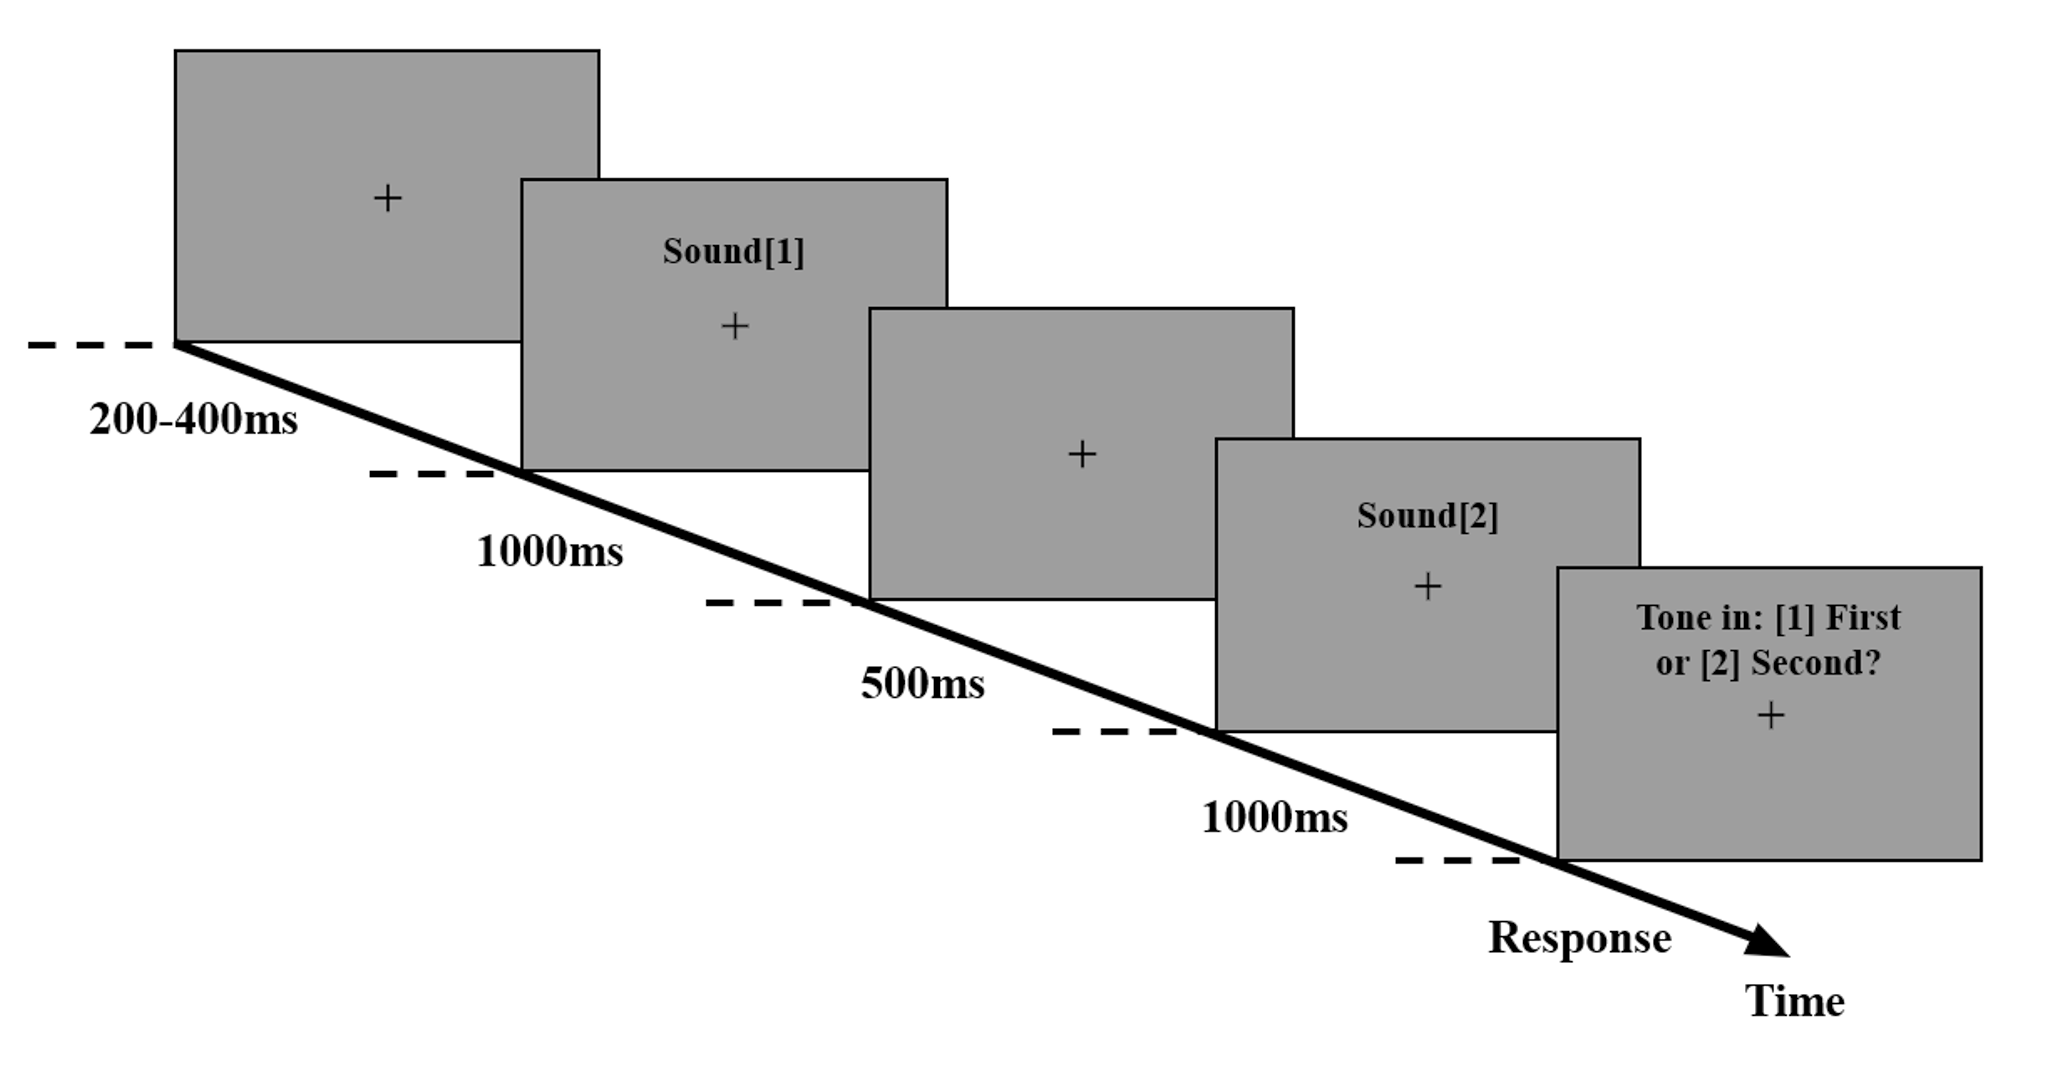
\includegraphics[width=0.9\textwidth]{figure/流程图.png}
    \captionsetup{labelsep=period}
    \caption{\small \rm 实验流程图。在每个试次中,首先呈现中央注视点200-400ms,接着会连续播放两段持续1s的噪声,噪音间隔500ms,纯音刺激会随机出现在一段噪音中。播放结束后显示反应提示语,被试需通过数字键1/2判断纯音出现在第一段噪音中还是第二段噪音中。}
    \label{fig:procedure}
\end{figure*}

\section{实\ 验\ 1}

\subsection{\heiti 被试}
\vspace{-1em}

实验1共招募了3名(2男1女)被试,均为浙江大学心理系22级本科生,年龄21-22岁,平均年龄21.3岁,被试均为右利手,无听力障碍,无过往神经或精神疾病史等。

\subsection{\heiti 仪器}
\vspace{-1em}

实验程序使用PsychoPy 2024.2.4 modern (py3.10) 编写。刺激通过开放式头戴耳机(飞利浦 X2HR)双耳呈现,耳机连接至一台个人电脑(Apple MacBook Air, M2 处理器)。被试在安静的房间内单独进行测试,使用标准计算机键盘记录反应。在实验开始前,所有被试的计算机系统音量输出均被手动设置为一个固定水平(最大音量的 1/16)。




\subsection{\heiti 刺激}
\vspace{-1em}
所有听觉刺激均以 16000 Hz 的采样率进行数字生成。掩蔽刺激为高斯白噪声,每个声音时长为 1000 毫秒。实验包含两种不同的噪音强度条件,其平均功率分别为 1.44 w和 0.64 w。目标信号为频率 1000 Hz、时长 100 毫秒的正弦纯音。为减少纯音前后的截断声,纯音的起始和结束部分采用了 20 毫秒的余弦斜坡(cosine ramp)进行包络。

每个试次中,纯音和噪音的功率比是使用 questplus 库中实现的 Quest+ 贝叶斯自适应心理物理过程\parencite{watson2017quest+} 来动态确定的。Quest+ 在线估计被试的心理测量函数参数(阈值、斜率、失误率),并为下一试次选择旨在提供最多信息的纯音/噪音功率比(P/N ratio)。给定试次的纯音绝对功率通过将 Quest+ 建议的功率比乘以该试次所用噪音掩蔽声的平均功率(1.44 w或 0.64 w)来计算。

\begin{figure*}[bp]
    \centering
    \begin{minipage}{0.342\textwidth}
        \centering
        \subcaption{}
        \vspace{-0.5em}
        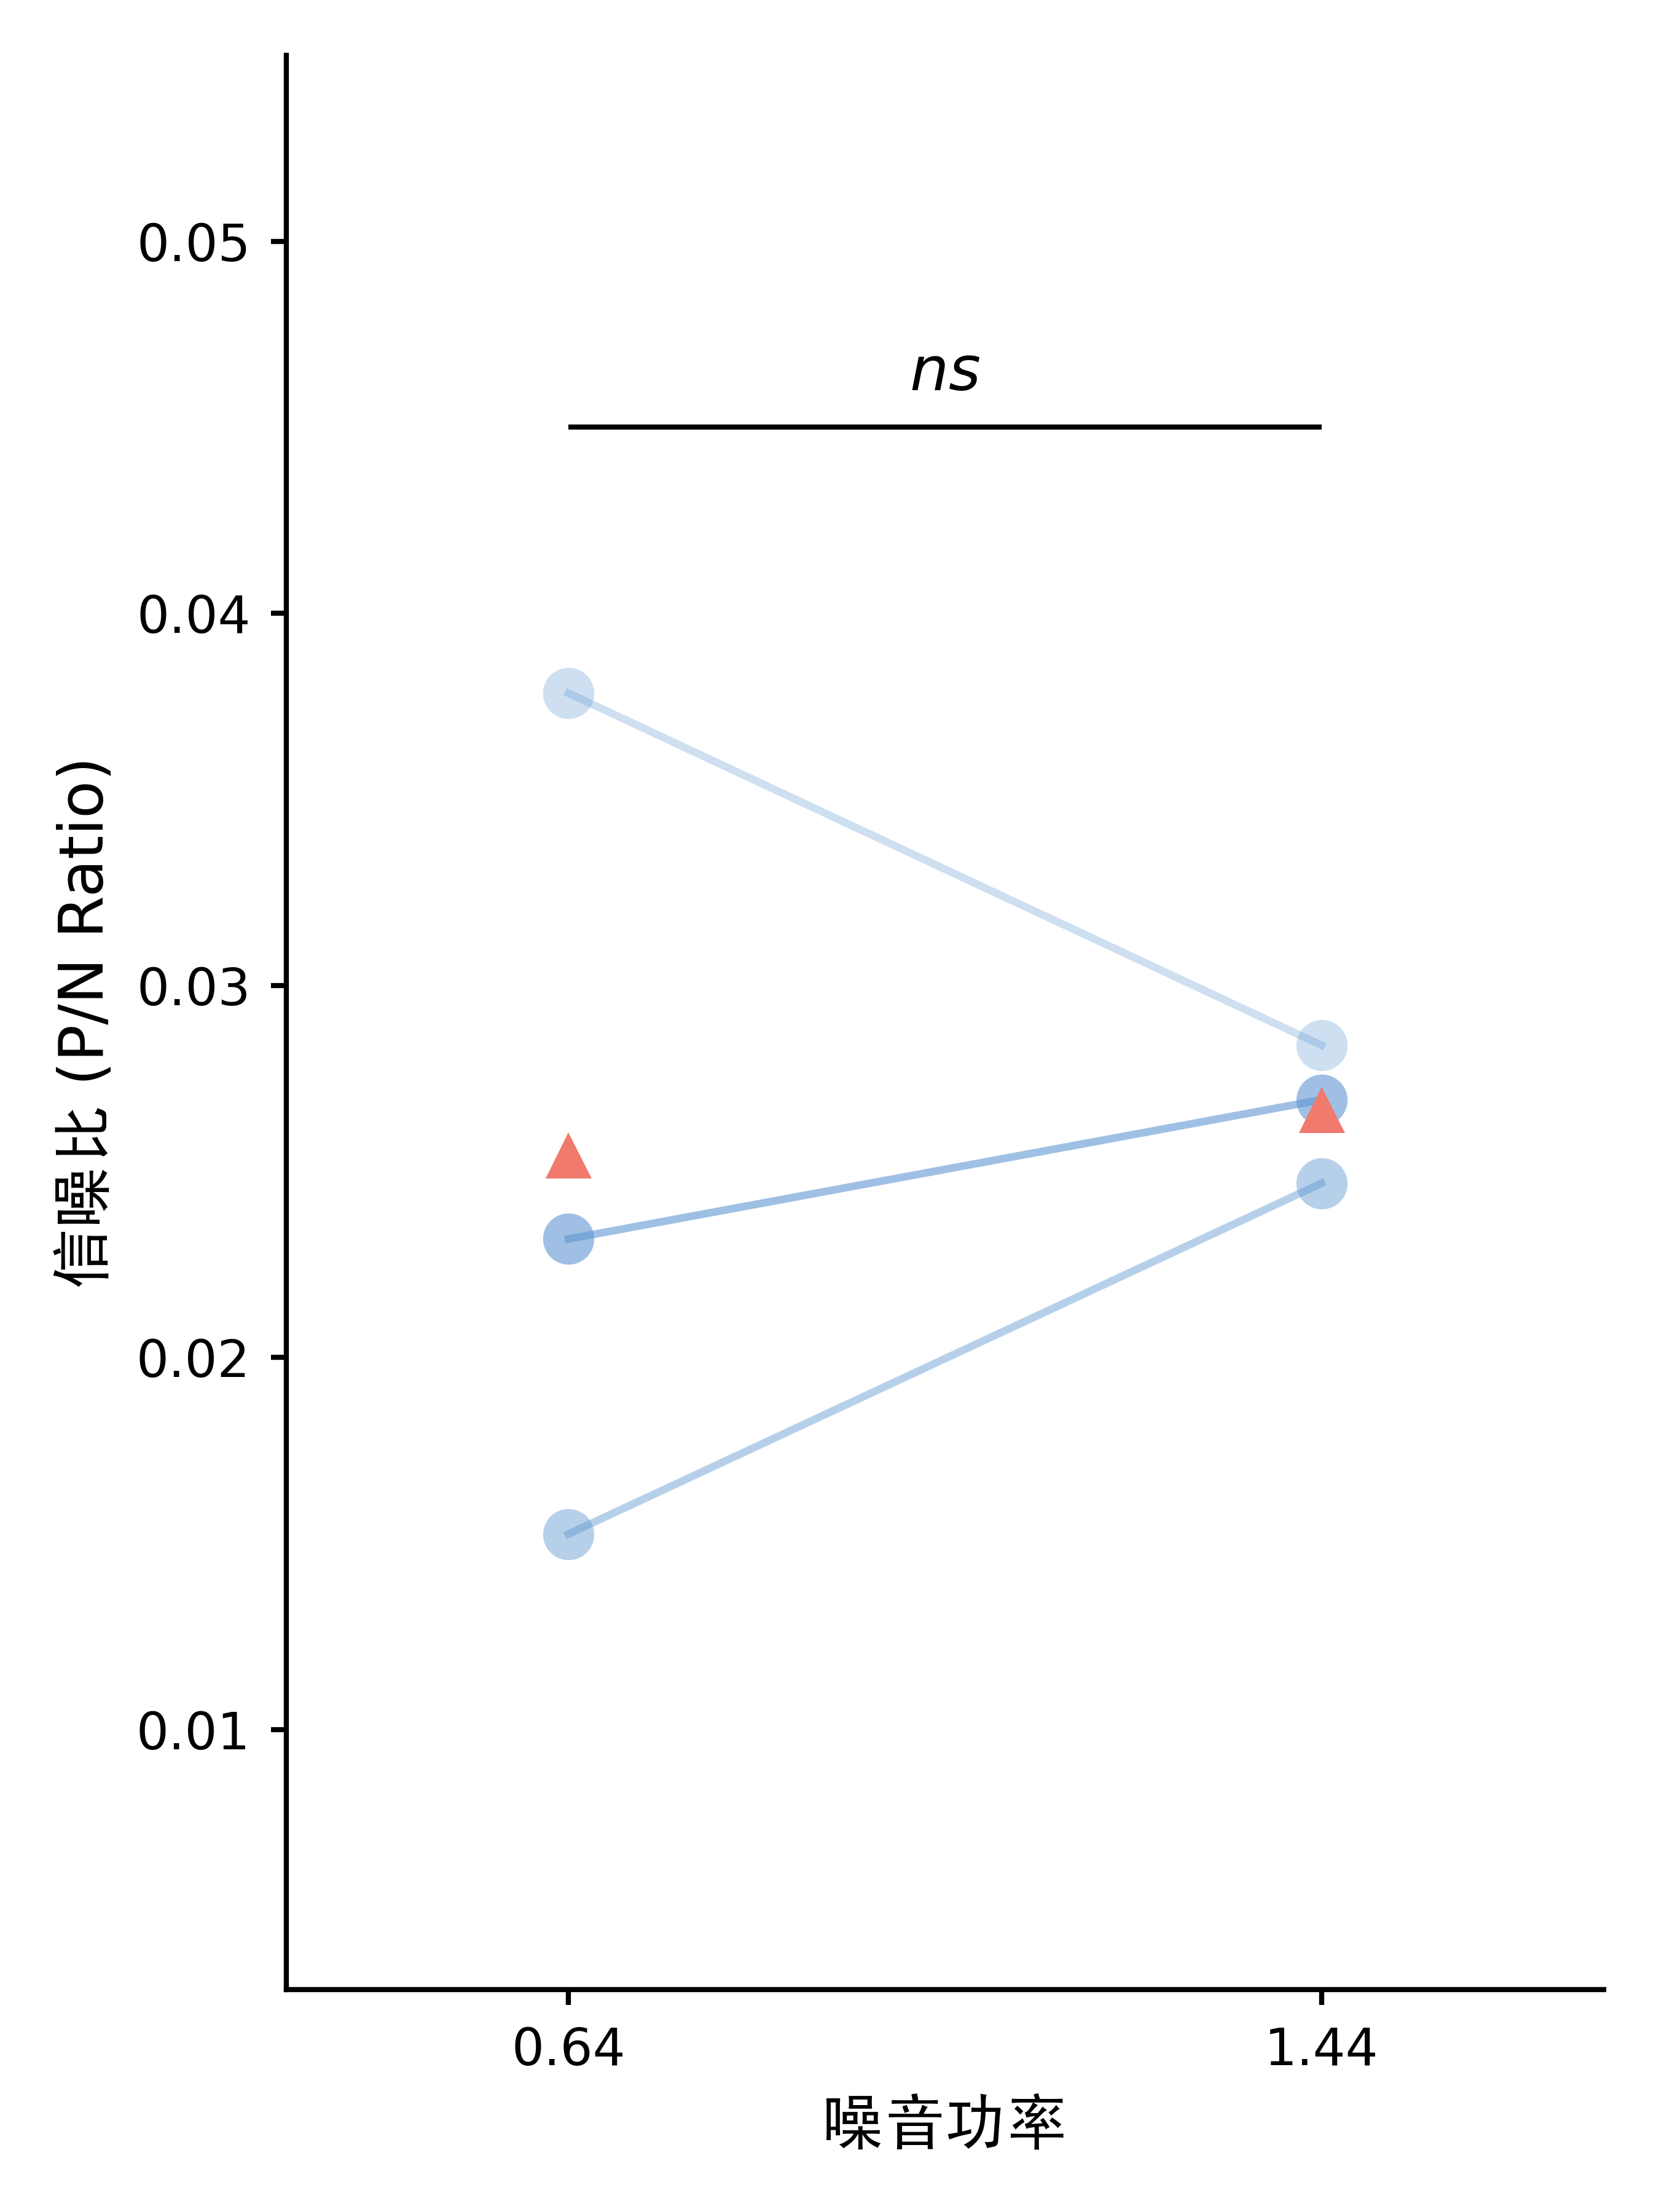
\includegraphics[width=\textwidth]{figure/ALL_participants_threshold_summary.png}
        \label{fig:exp1}
    \end{minipage}
    \begin{minipage}{0.608\textwidth}
        \centering
        \subcaption{}
        \vspace{-0.5em}
        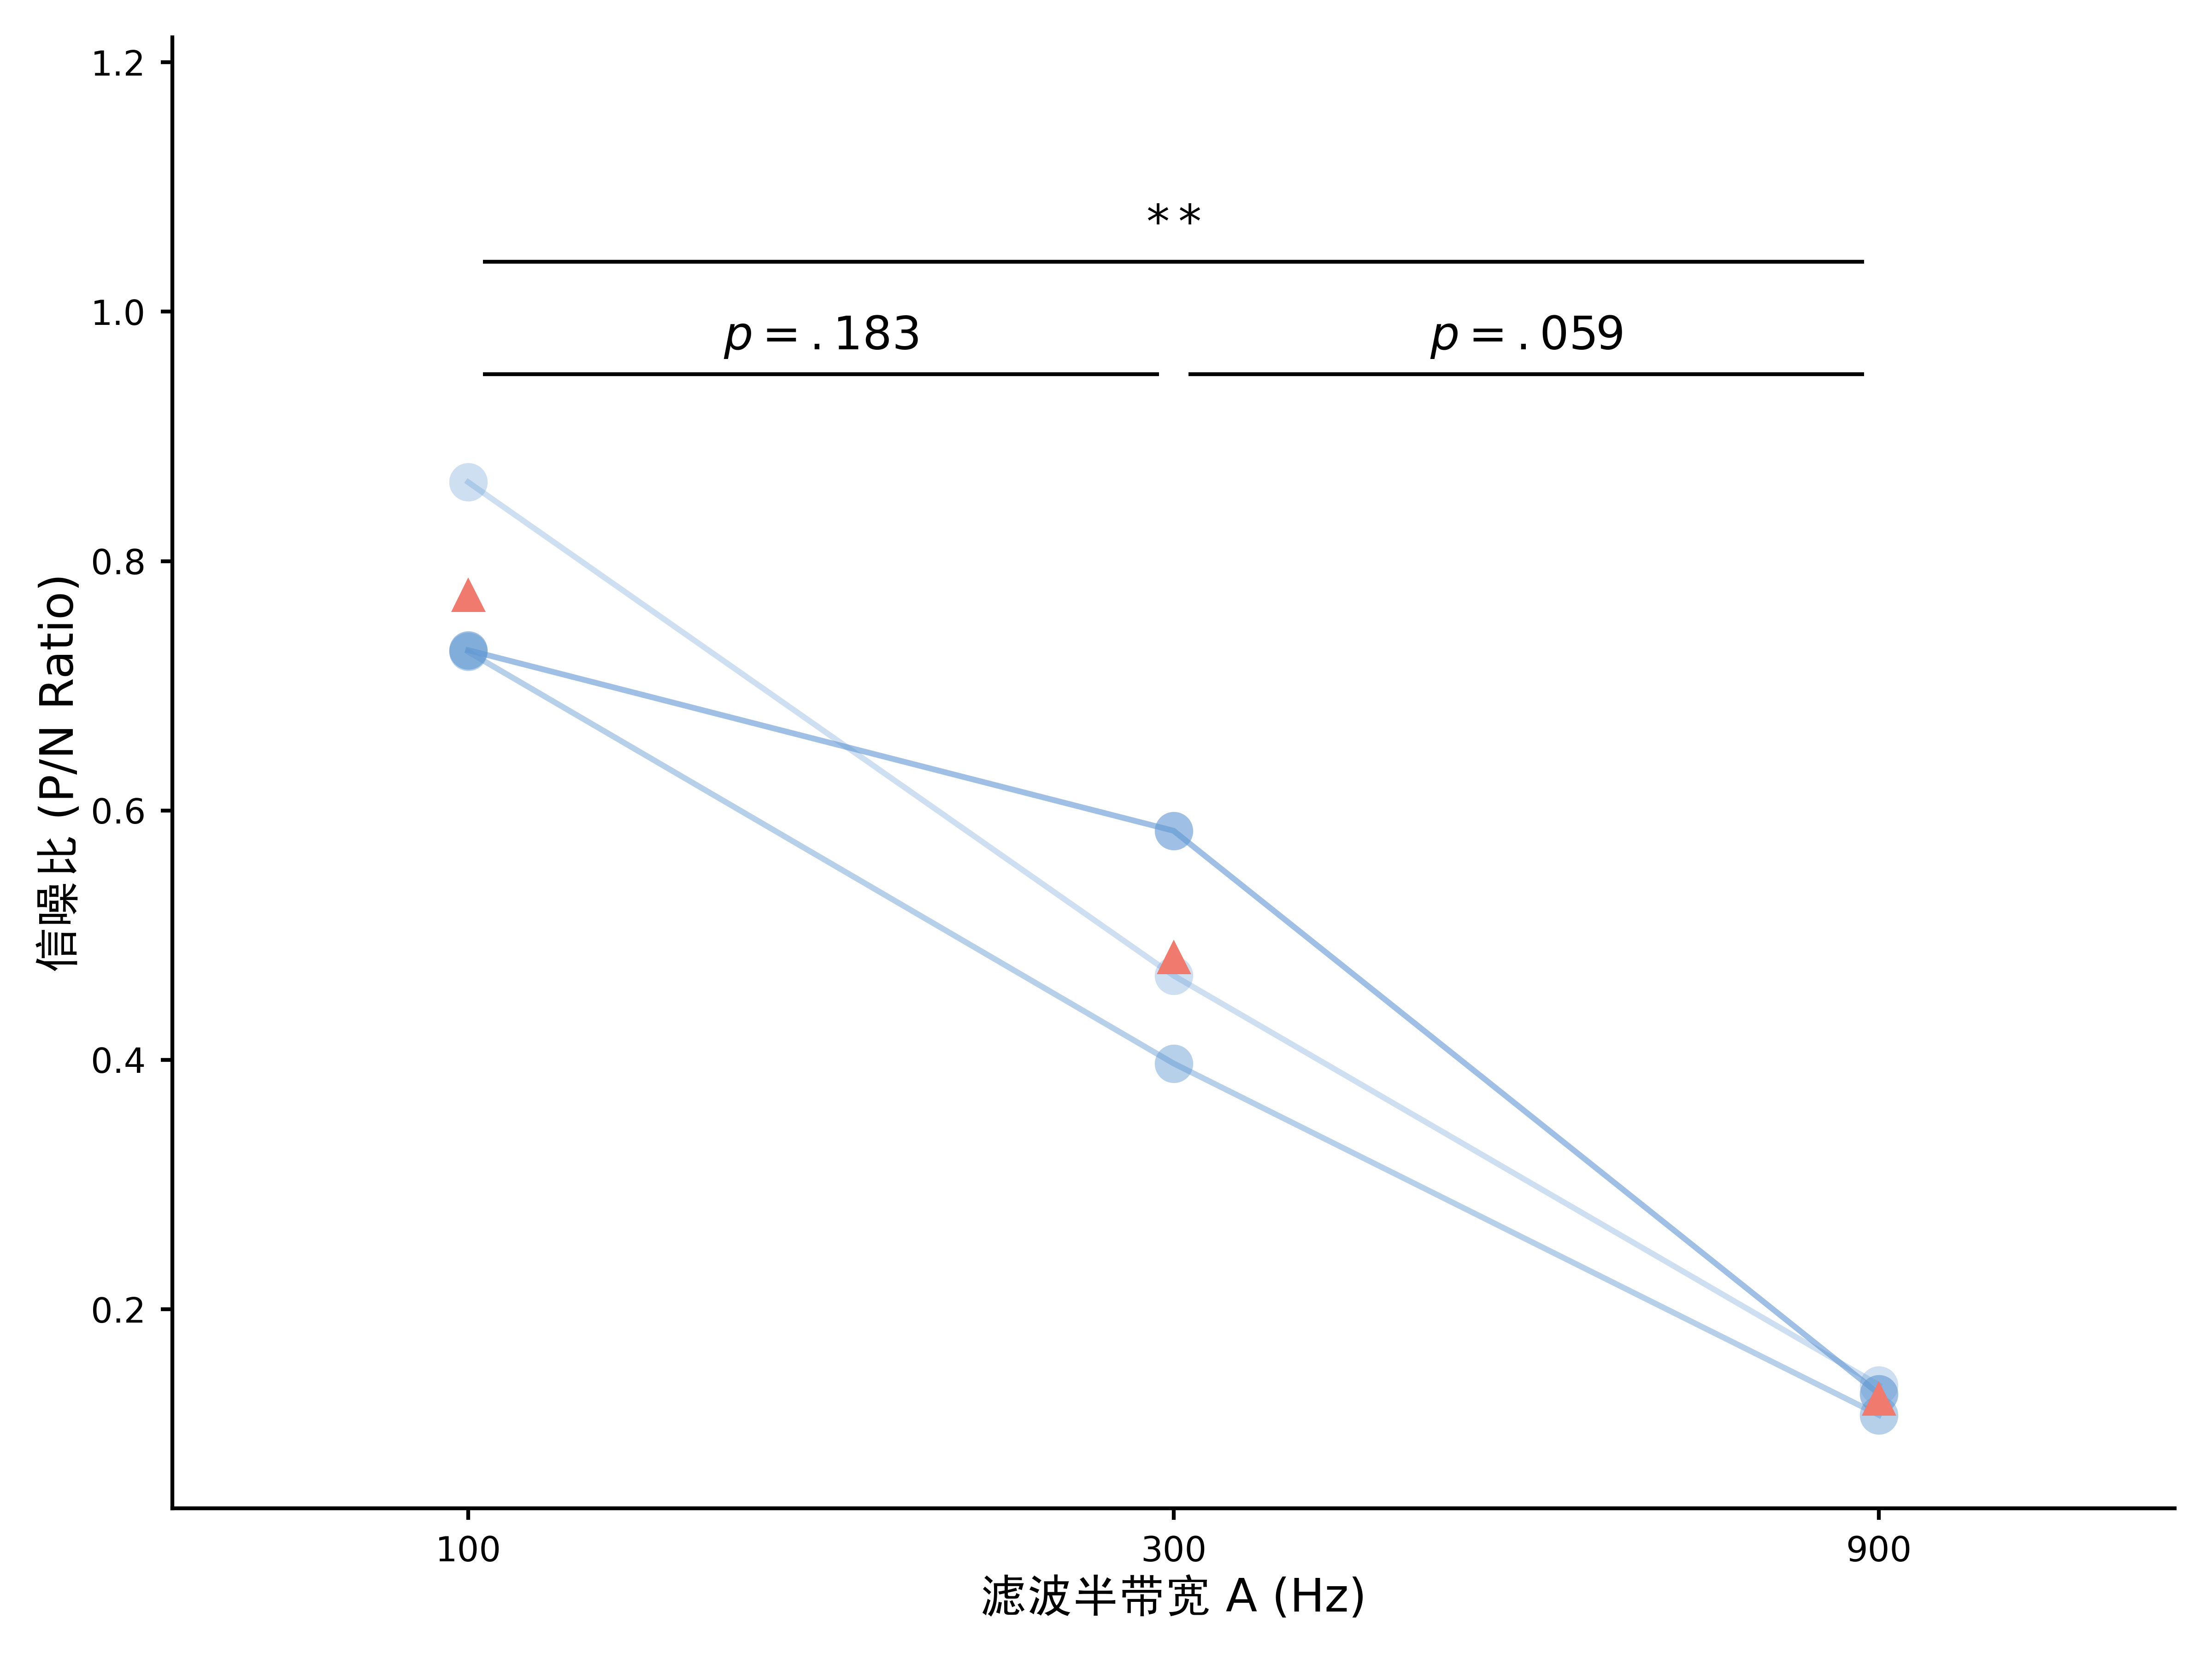
\includegraphics[width=\textwidth]{figure/EXP2_BW_ALL_participants_threshold_summary.png}
        \label{fig:exp2plot}
    \end{minipage}
    \captionsetup{labelsep=period}
    \caption{\small \rm a) 实验1结果图。图中的青色实心圆点是每个被试的统计值,同一被试用实线相连。橙色三角形是所有被试的平均值。横轴是噪声的两个能量水平,纵轴是纯音和噪音的功率比值。b) 实验2结果图,图中的青色实心圆点是每个被试的统计值,同一被试用实线相连。青色三角形是所有被试的平均值。横轴是滤波器半带宽A的三个水平,纵轴是纯音和噪音的功率比值。\\
    注:**:\(p<.01\)}
\end{figure*}

\subsection{\heiti 流程}
\vspace{-1em}
实验1的实验流程如Figure\ref{fig:procedure}所示。在每个试次中,首先呈现中央注视点200-400ms,接着会连续播放两段持续1s的噪声,噪音间隔500ms。噪音绝对功率随机(0.64w或1.44w),但一个试次中两段噪音绝对功率相同。纯音刺激会随机出现在一段噪音中,并在噪音播放500ms开始,持续100ms。噪声播放结束后显示反应提示语``Tone in: [1] First or [2] Second?'',被试需通过数字键1/2判断纯音出现在第一段噪音中还是第二段噪音中。待被试按键反应后,间隔300ms后进入下一试次。实验共包含6个练习试次(每种噪声条件3次)和64个正式试次(每种噪声条件32次),每个block32个试次,共2个block,block之间休息1分钟,总用时约6-7分钟。


\subsection{\heiti 结果}
\vspace{-1em}

高、低两种噪音水平(平均功率分别为1.44w和0.64w)条件下的纯音阈值(以纯音与噪声平均功率的比值P/N Ratio表示)见Figure\ref{fig:exp1}。

在每种噪音条件下,被试对纯音刺激的听觉阈值由Quest+算法给出,计算方法为P/N Ratio的后验概率密度分布的期望值。为了检验\(H_1\)(掩蔽噪音强度的主效应显著),采用配对样本t检验比较了两种噪音水平下的纯音阈值。结果显示,高噪音水平与低噪音水平条件下的纯音阈值差异不显著,\(t\)(2) = 0.22, \(p\) > 0.05。

为进一步评估证据强度,我们进行了贝叶斯配对样本t检验,数据分析通过JASP 0.19.3软件完成。结果表明, \(BF_{01}\)= 2.09,表明支持零假设(噪音强度无主效应)的证据强度是支持备择假设(噪音强度存在主效应)的2.09倍。根据Jeffreys (1961) 的分类标准,这为零假设提供了较弱的证据。因此,实验1的结果未能支持\(H_1\),即未发现纯音阈值随噪音强度增大而显著升高的现象。




\section{实\ 验\ 2}

\subsection{\heiti 被试}
\vspace{-1em}

实验2的被试和实验1相同。

\subsection{\heiti 仪器}
\vspace{-1em}

硬件设备、被试设置、反应方式以及系统音量输出设置均与实验1相同。其中,数字信号滤波处理使用SciPy库进行。

\subsection{\heiti 刺激}
\vspace{-1em}

所有听觉刺激均以 16000 Hz 的采样率进行数字生成。掩蔽刺激通过高斯白噪声(时长 1000 毫秒)处理得到。首先生成一段高斯白噪音,随后使用一个中心频率为 1000 Hz 的数字带通滤波器进行处理。实验测试了三种滤波器带宽条件,由半带宽参数 A 定义,其值分别为 100 Hz、300 Hz 和 900 Hz。这些条件分别对应 900–1100 Hz、700–1300 Hz 和 100–1900 Hz 的滤波器通带。滤波通过一个使用汉明窗(Hamming window)设计的 64 阶有限脉冲响应(FIR)滤波器实现。由于相等功率的噪音在不同的滤波处理后,功率会发生变化,因此处理后的噪音信号均被标准化,使其均方根(RMS)幅值为 1.0。这确保了在所有三种带宽条件下,噪音掩蔽声的平均功率恒定为 1.0。目标信号和实验1相同,为频率 1000 Hz、时长 100 毫秒的正弦纯音。为减少纯音前后的截断声,纯音的起始和结束部分采用了 20 毫秒的余弦斜坡(cosine ramp)进行包络。

和实验1相同,每个试次中纯音和噪音的功率比是使用 questplus 库中实现的 Quest+ 贝叶斯自适应心理物理过程来动态确定的。

\begin{figure*}[!t]
    \centering
    \includegraphics[width = 0.9\textwidth]{figure/questplot.png}
    \captionsetup{labelsep=period}
    \caption{\small \rm 不同条件下信噪比随实验进行的变化。三种条件下初始化信噪比都为1.2。图中的折线是所有被试的平均值的滑动平均(窗口大小为5个试次),每个试次的标准误也是以5个试次为窗口大小,计算五个试次的信噪比的标准差得到的。可以发现,随着实验的进行,信噪比变化的幅度之间减小,斜率逐渐平缓,说明后验分布逐渐趋于稳定。}
    \label{fig:quest}
\end{figure*}

\subsection{\heiti 结果}
\vspace{-1em}

实验2操纵了带通滤波器的半带宽A,设置了三个水平:100 Hz, 300 Hz, 900 Hz。Figure\ref{fig:exp2plot}展示了不同滤波器半带宽A条件下的纯音阈值(P/N Ratio),Figure\ref{fig:quest}展示了不同条件下纯音阈值随实验进行的收敛情况。

为了检验\(H_2\),采用单因素重复测量方差分析(ANOVA)对三个滤波器半带宽水平下的纯音阈值进行了比较。Mauchly球形检验结果显示数据满足球形假设,\(\rm \chi^2\)(2) = 0.80, \(p\) = 0.67。ANOVA结果显示,滤波器半带宽A的主效应显著,\(F\)(2, 4) = 63.60, \(p\) = 0.001, \(\rm \eta_p^2\) = 0.970。

事后两两比较采用Bonferroni校正。结果显示:A=100 Hz (\(M\) = 0.77) 与 A=900 Hz (\(M\) = 0.12) 条件下的纯音阈值差异显著(\(p\) = 0.012);A=300 Hz (\(M\) = 0.48) 与 A=900 Hz 条件下的差异达到边缘显著水平(\(p\) = 0.059);而 A=100 Hz 与 A=300 Hz 条件下的差异不显著(\(p\) = 0.183)。

为进一步探究阈值随带宽变化的模式,我们进行了趋势分析。结果表明,纯音阈值(PNRatio)随着滤波器半带宽A的增加呈现显著的线性下降趋势,\(F\)(1, 2) = 256.58, \(p\) = 0.004, \(\rm \eta_p^2\) = 0.992。二次趋势不显著,\(F\)(1, 2) = 0.28, \(p\) = 0.652, \(\rm \eta_p^2\)  = 0.121。

贝叶斯重复测量方差分析分析结果进一步印证了上述发现。仅包含滤波器半带宽主效应的模型得到了数据极强的证据支持(\(BF_{10}\) = 167.94);而仅包含被试差异主效应的模型\(BF_{10}\) = 0.400)。这表明滤波器半带宽是影响纯音阈值的主要因素,被试间的个体差异对模型解释的贡献不显著。

综合来看,实验2的结果基本支持\(H_2\),表明滤波器半带宽A显著影响噪音掩蔽下的纯音阈值,且随着半带宽A的增大,纯音阈值(P/N Ratio)呈现下降趋势,尤其在从较窄带宽向最宽带宽(900 Hz)变化时,下降幅度更为明显。




% \begin{figure*}[!htb]
%     \centering
%     % 第一行子图
%     \begin{minipage}{0.49\textwidth}
%         \centering
%         \subcaption{}
%         \vspace{-0.5em}
%         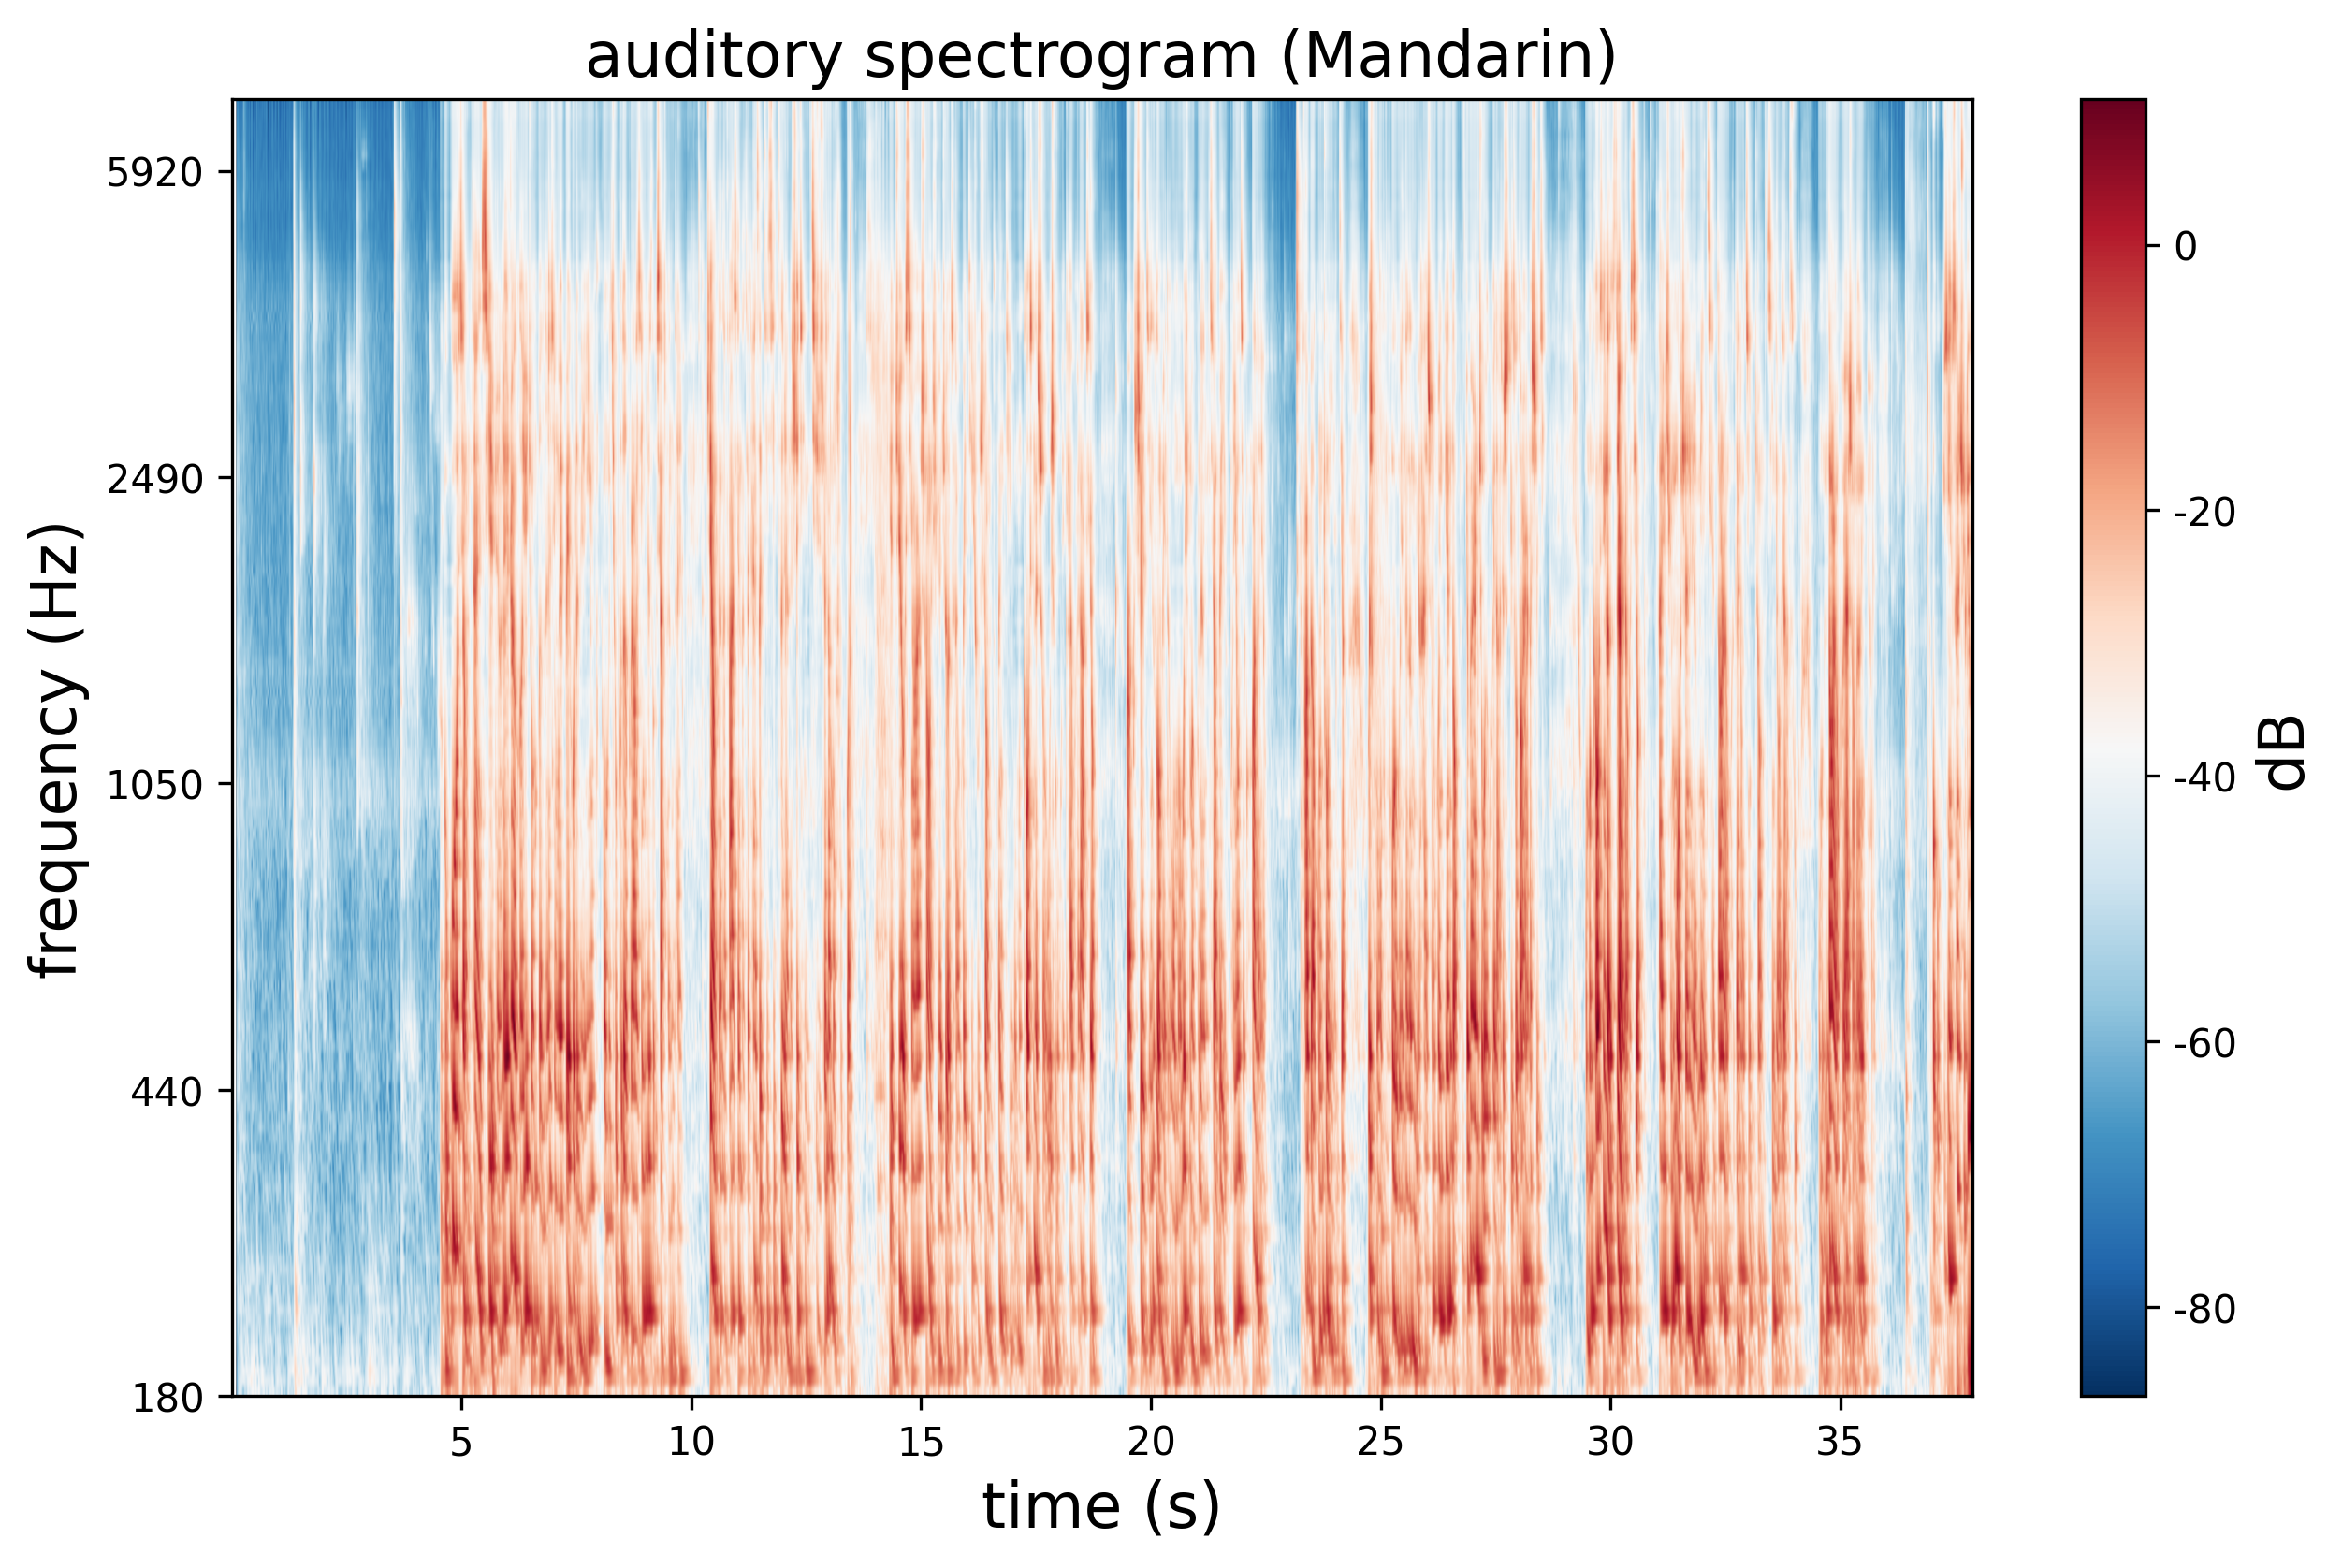
\includegraphics[width=\textwidth]{figure/shuohua.png}
%         \label{spectrogram:shuohua}
%     \end{minipage}
%     \begin{minipage}{0.49\textwidth}
%         \centering
%         \subcaption{}
%         \vspace{-0.5em}
%         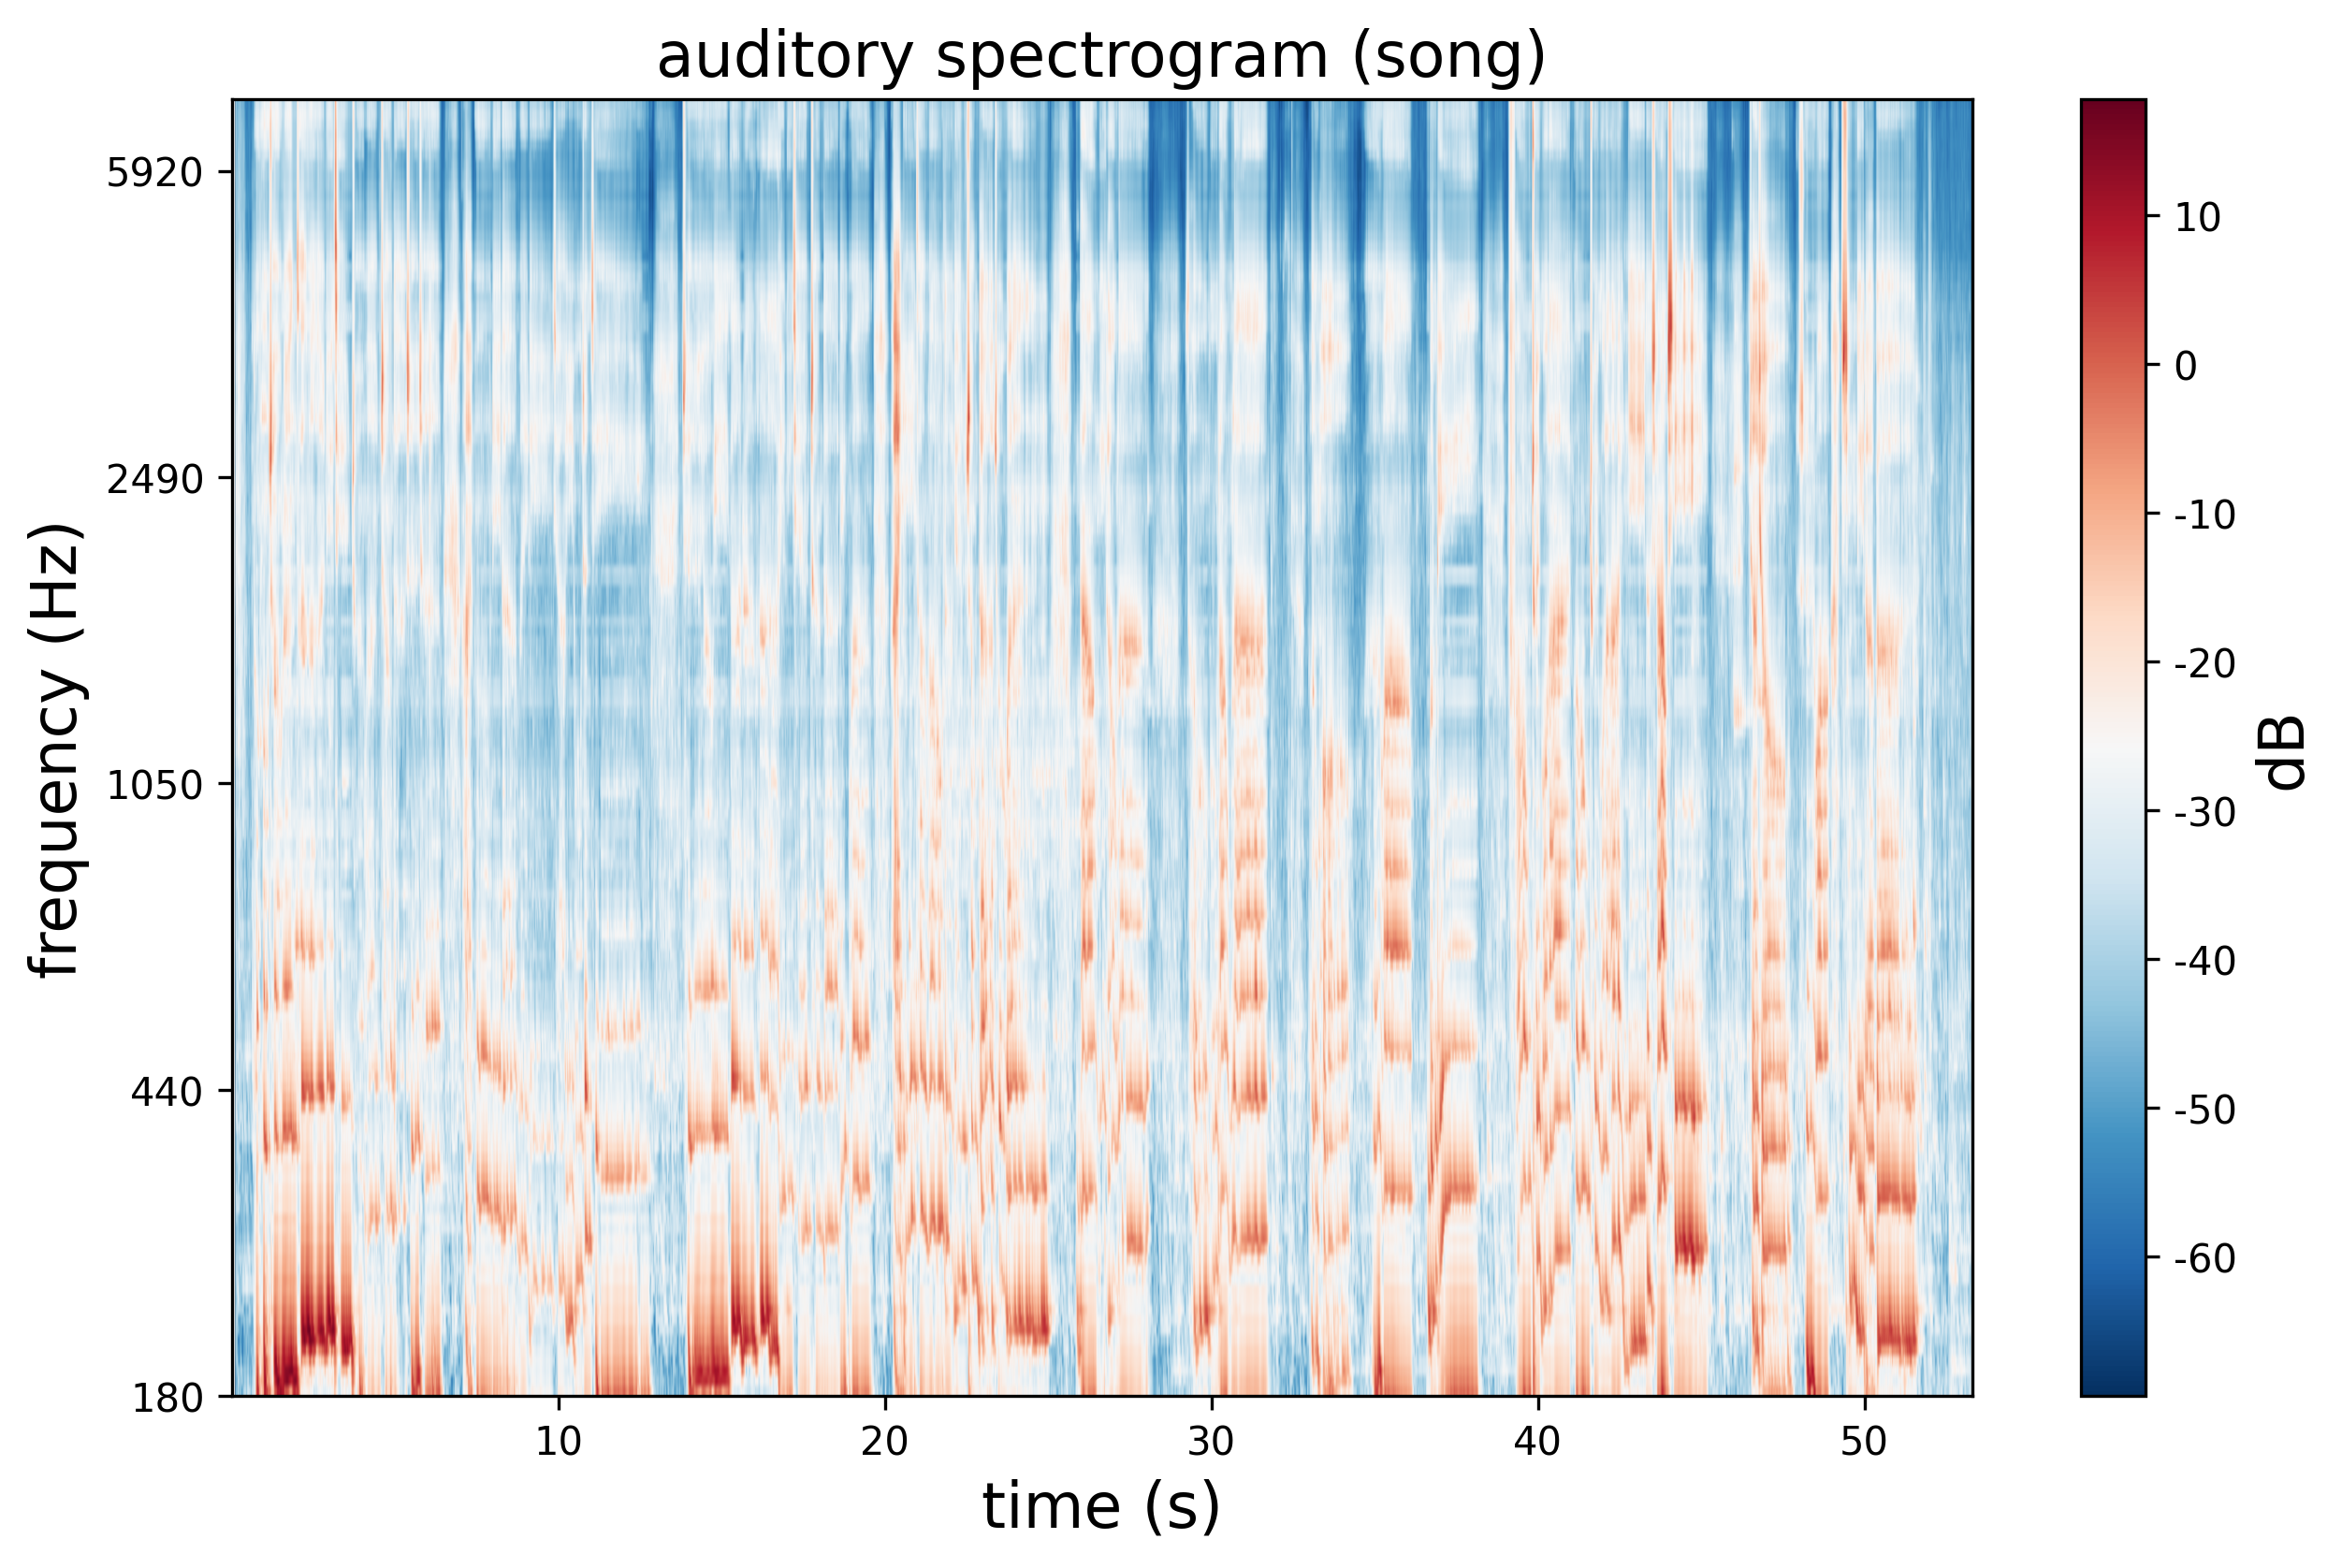
\includegraphics[width=\textwidth]{figure/song.png}
%         \label{spectrogram:song}
%     \end{minipage}
    
%     \vspace{-2em} % 调整两行子图之间的间距
    
%     % 第二行子图
%     \begin{minipage}{0.49\textwidth}
%         \centering
%         \subcaption{}
%         \vspace{-0.5em}
%         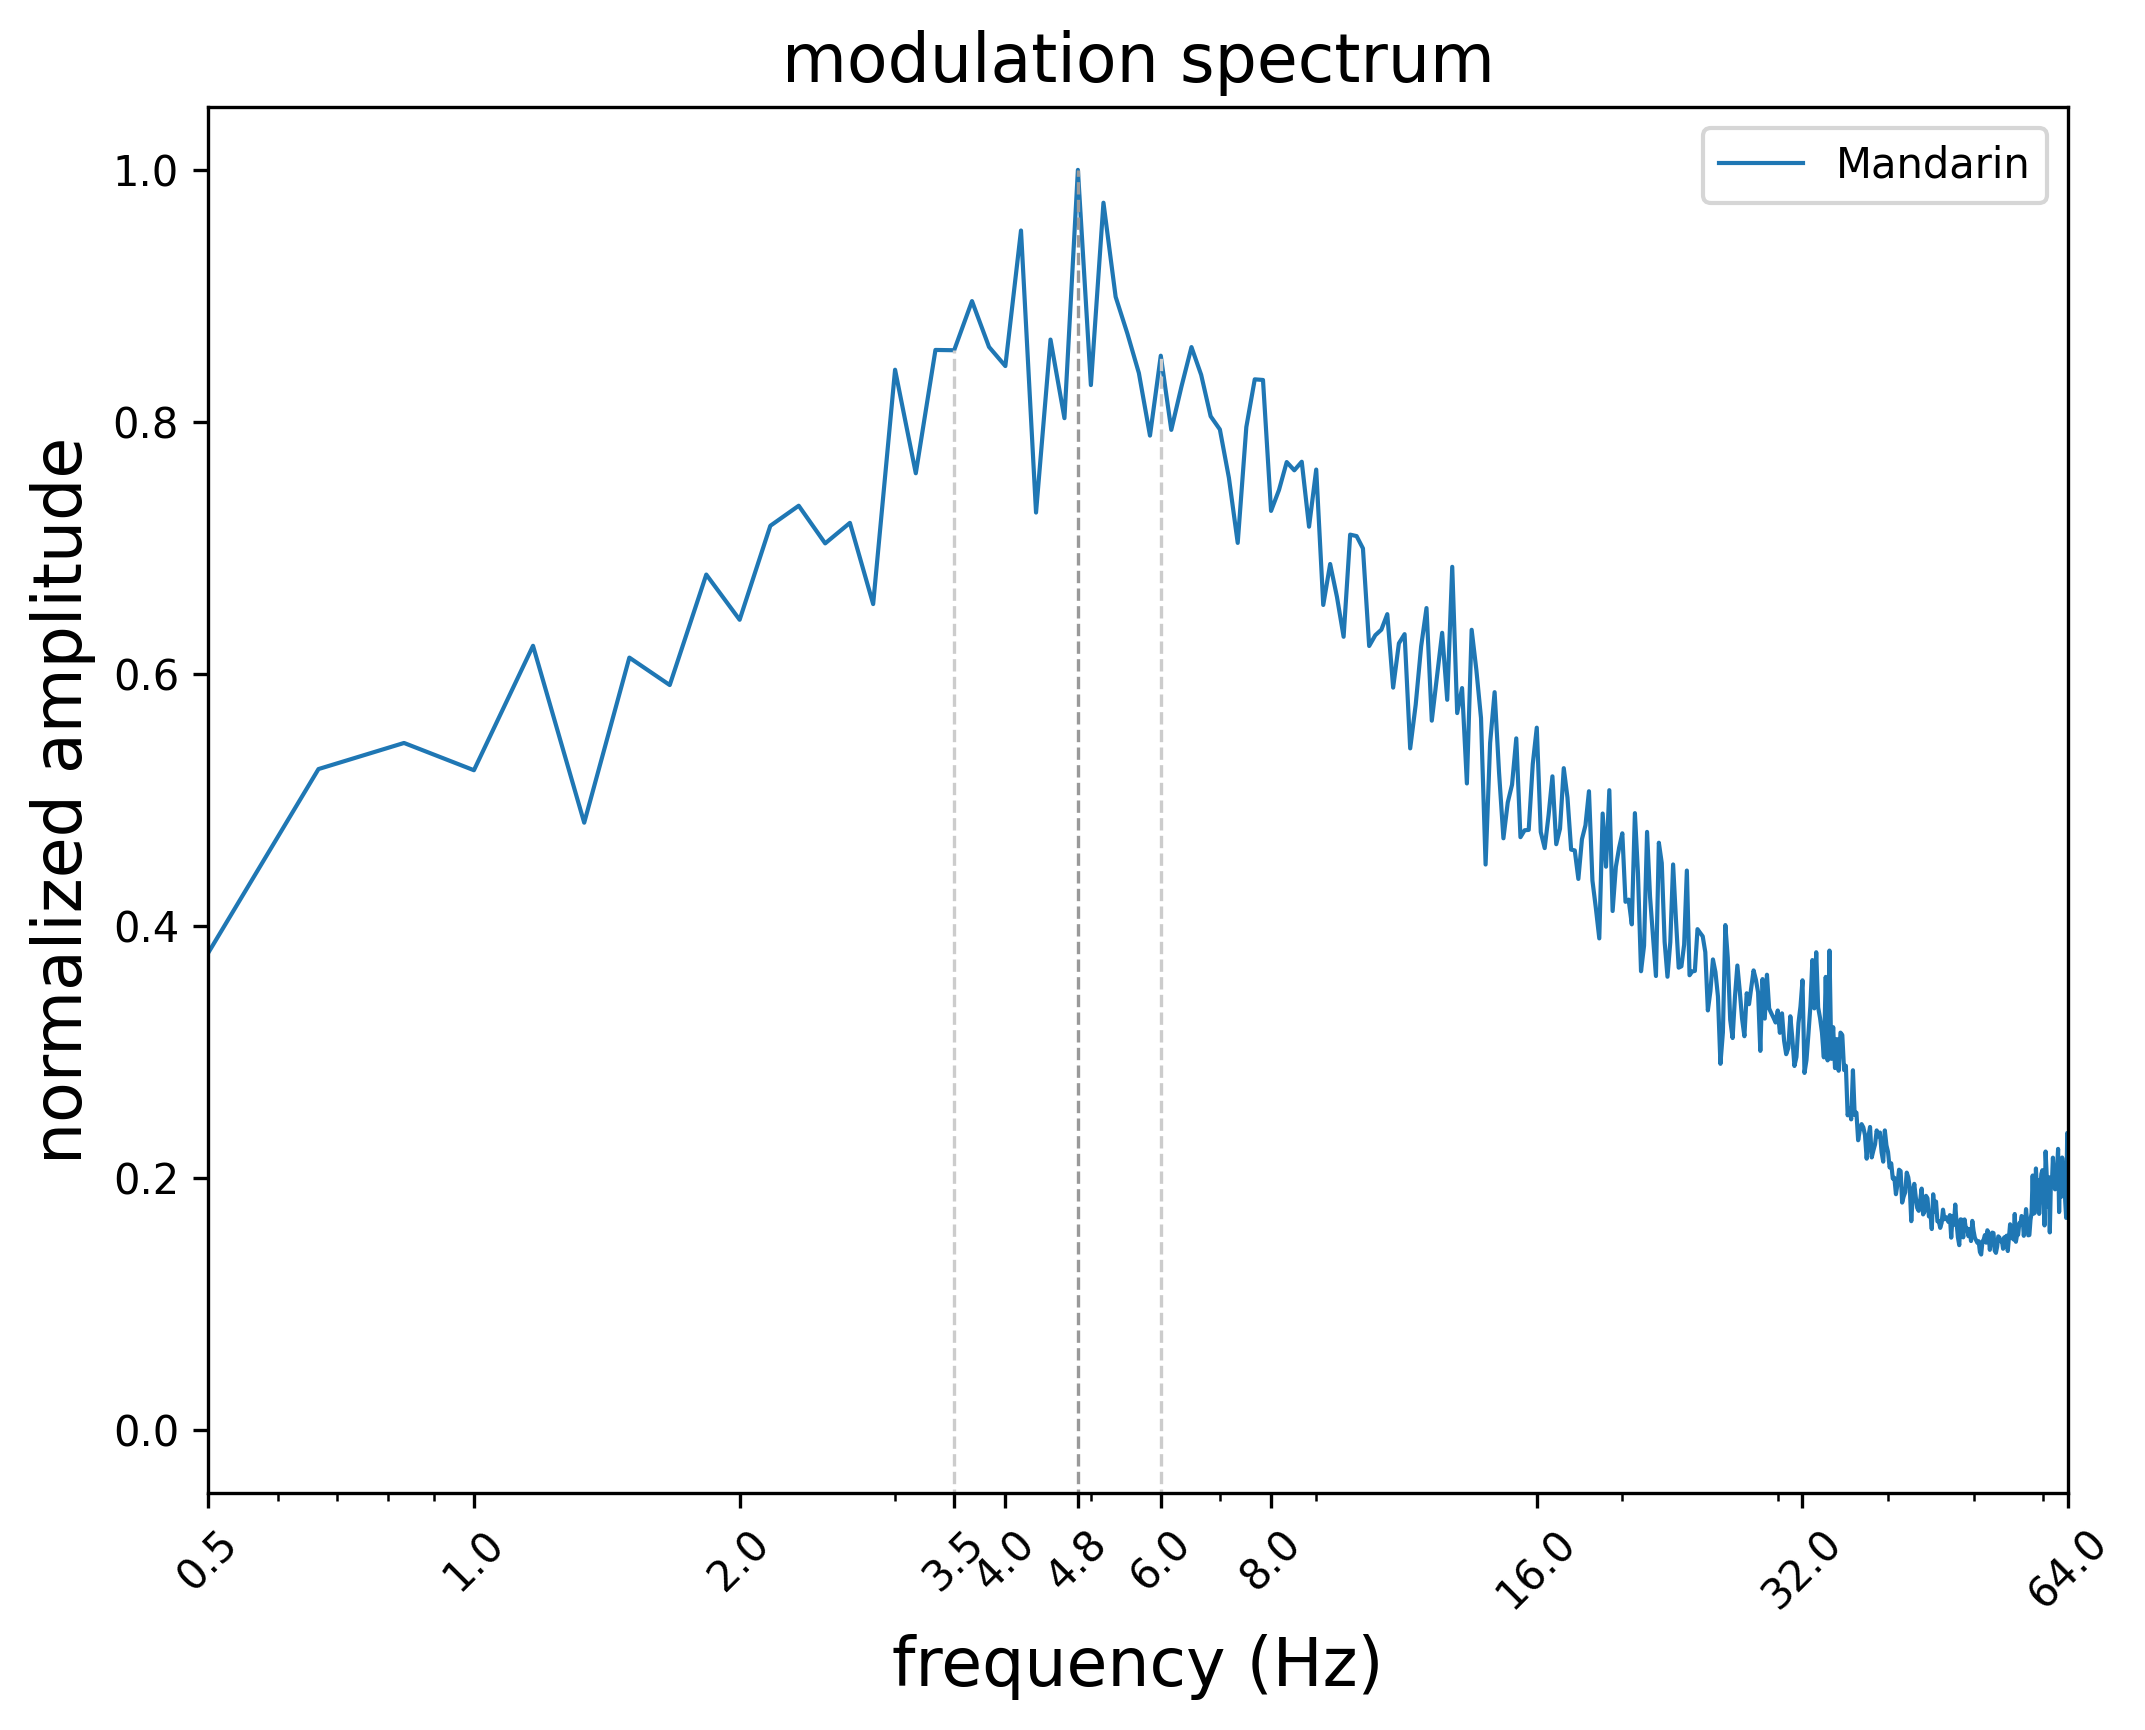
\includegraphics[width=\textwidth]{figure/spectrum_shuohua.png}
%         \label{spectrum:shuohua}
%     \end{minipage}
%     \begin{minipage}{0.49\textwidth}
%         \centering
%         \subcaption{}
%         \vspace{-0.5em}
%         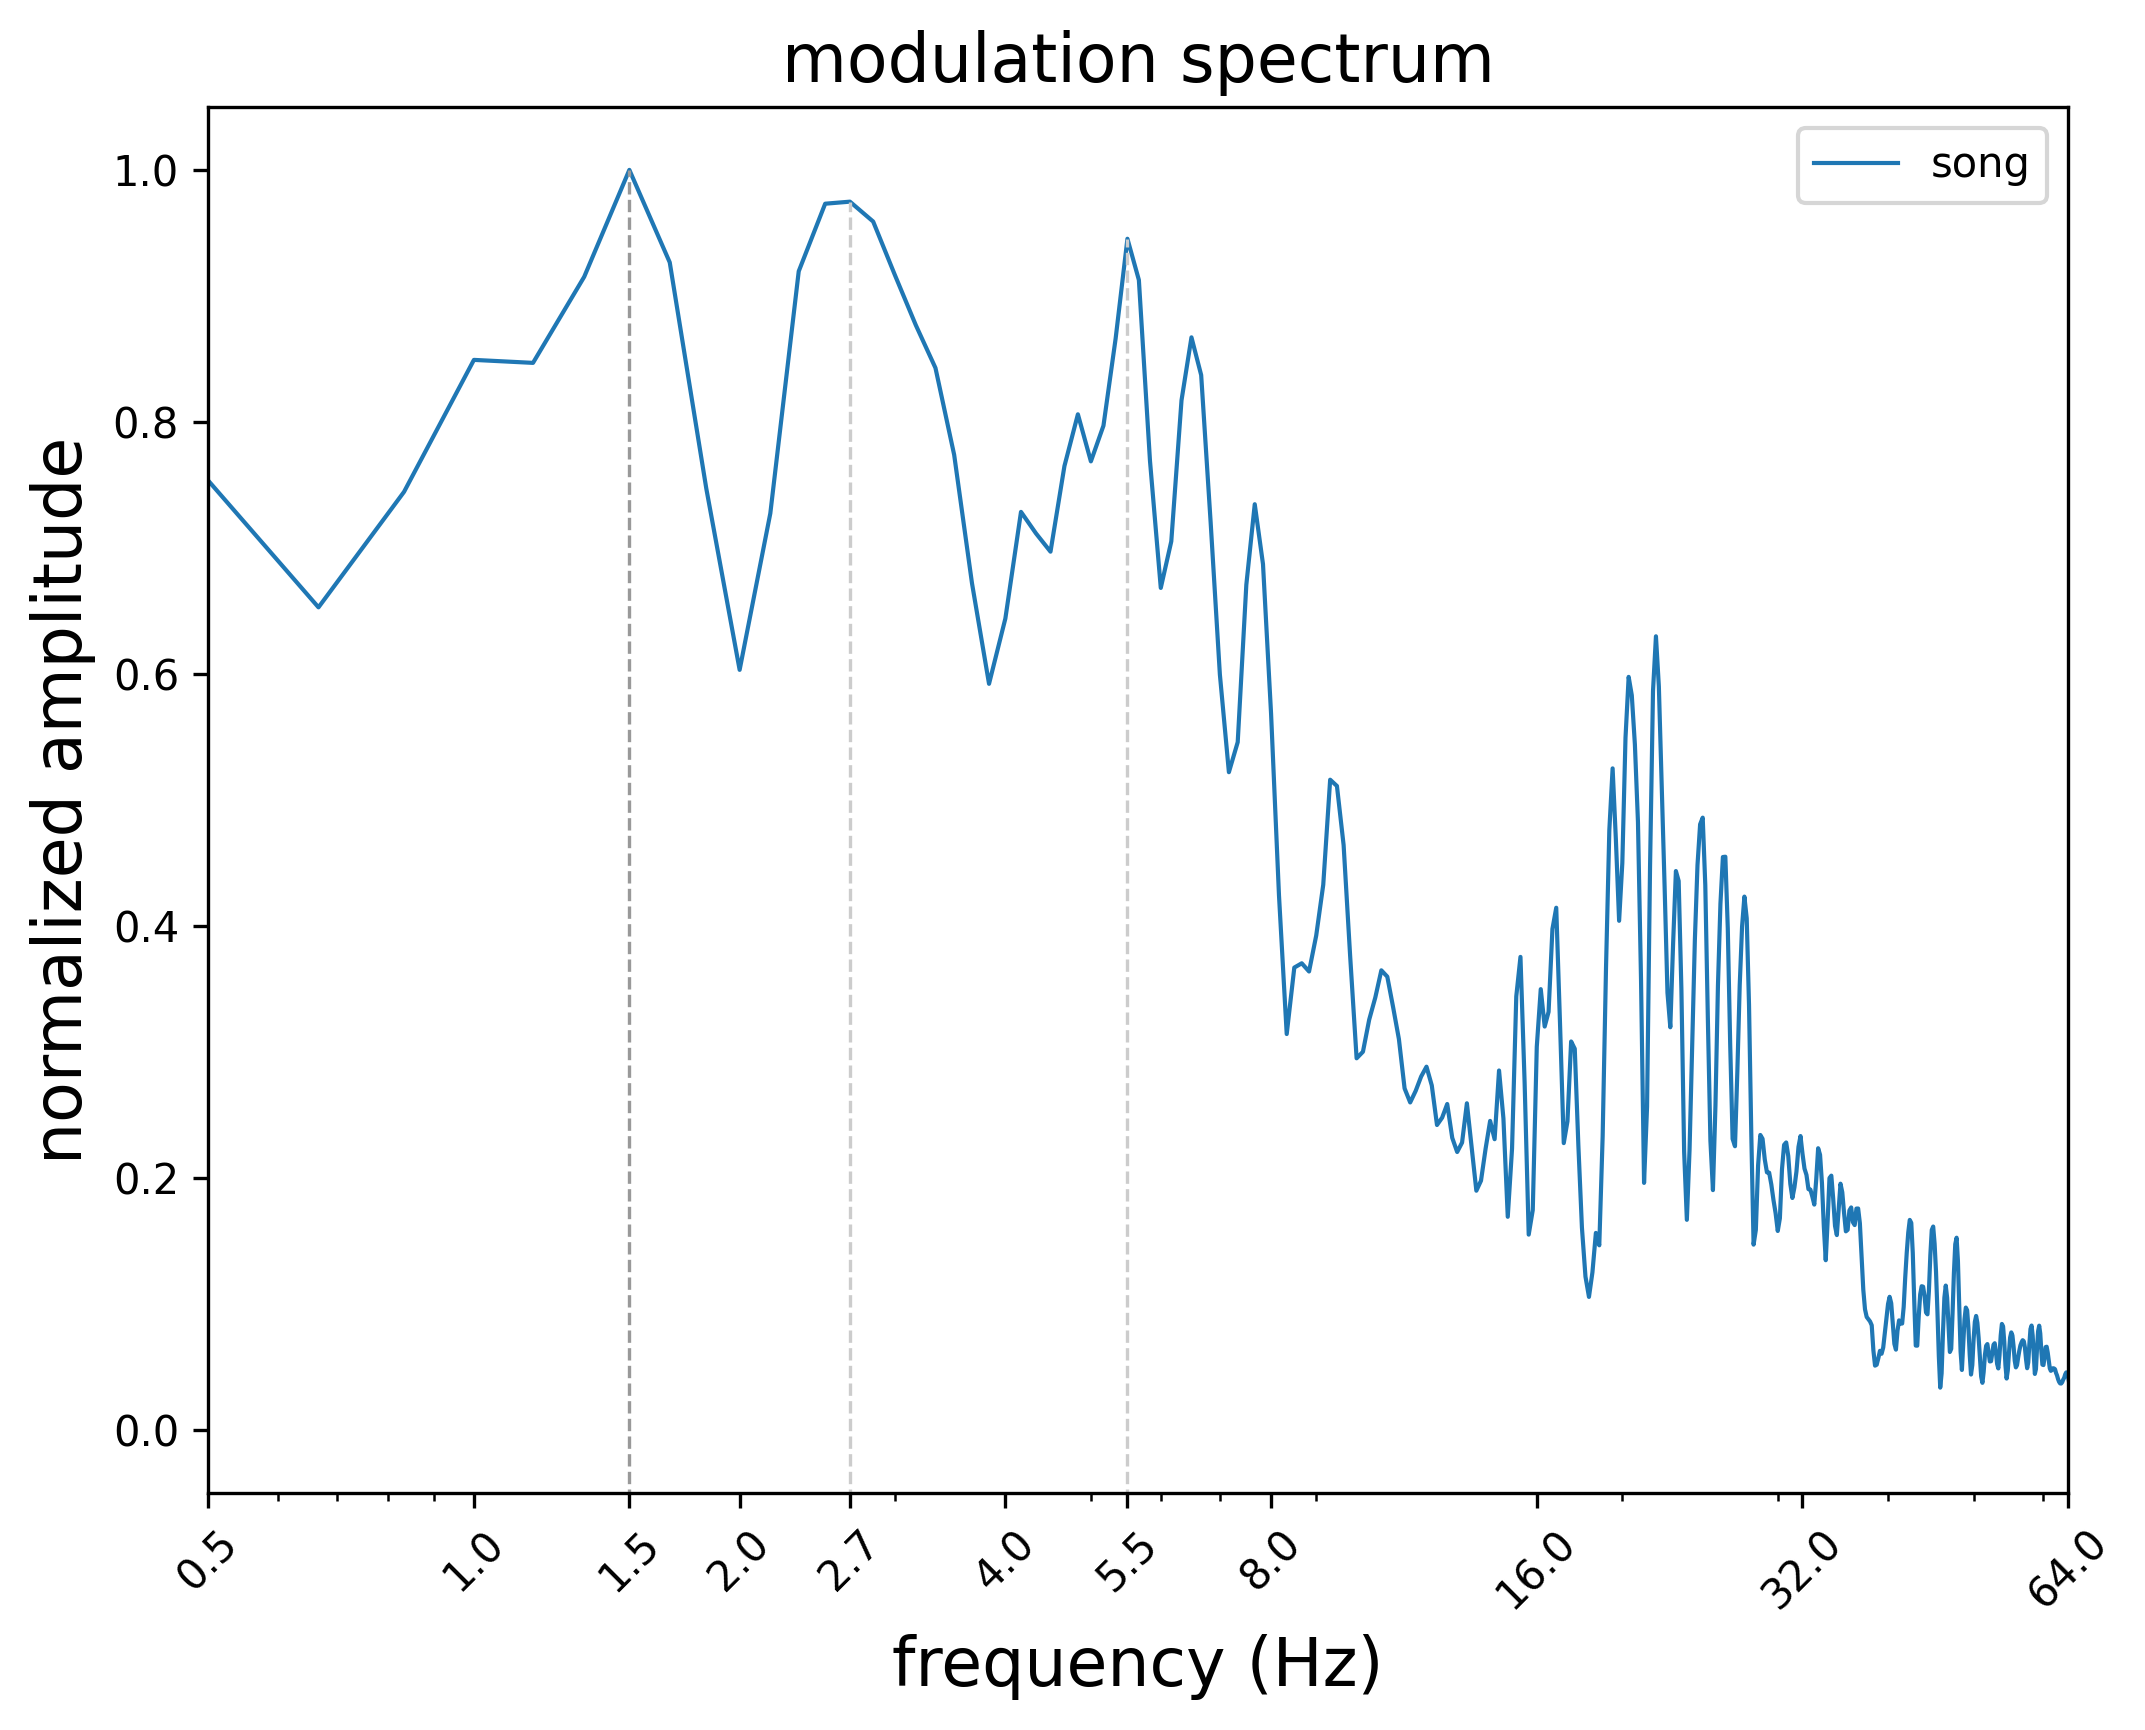
\includegraphics[width=\textwidth]{figure/spectrum_song.png}
%         \label{spectrum:song}
%     \end{minipage}
    
%     \captionsetup{labelsep=period}
%     \vspace{-1em}
%     \caption{\small 个人普通话语音和歌唱的时频图和调制谱}
    
%     \label{fig:fig1}
% \end{figure*}


% \begin{figure*}[!htb]
%     \centering
%     % 第一行子图
%     \begin{minipage}{0.49\textwidth}
%         \centering
%         \subcaption{}
%         \vspace{-0.5em}
%         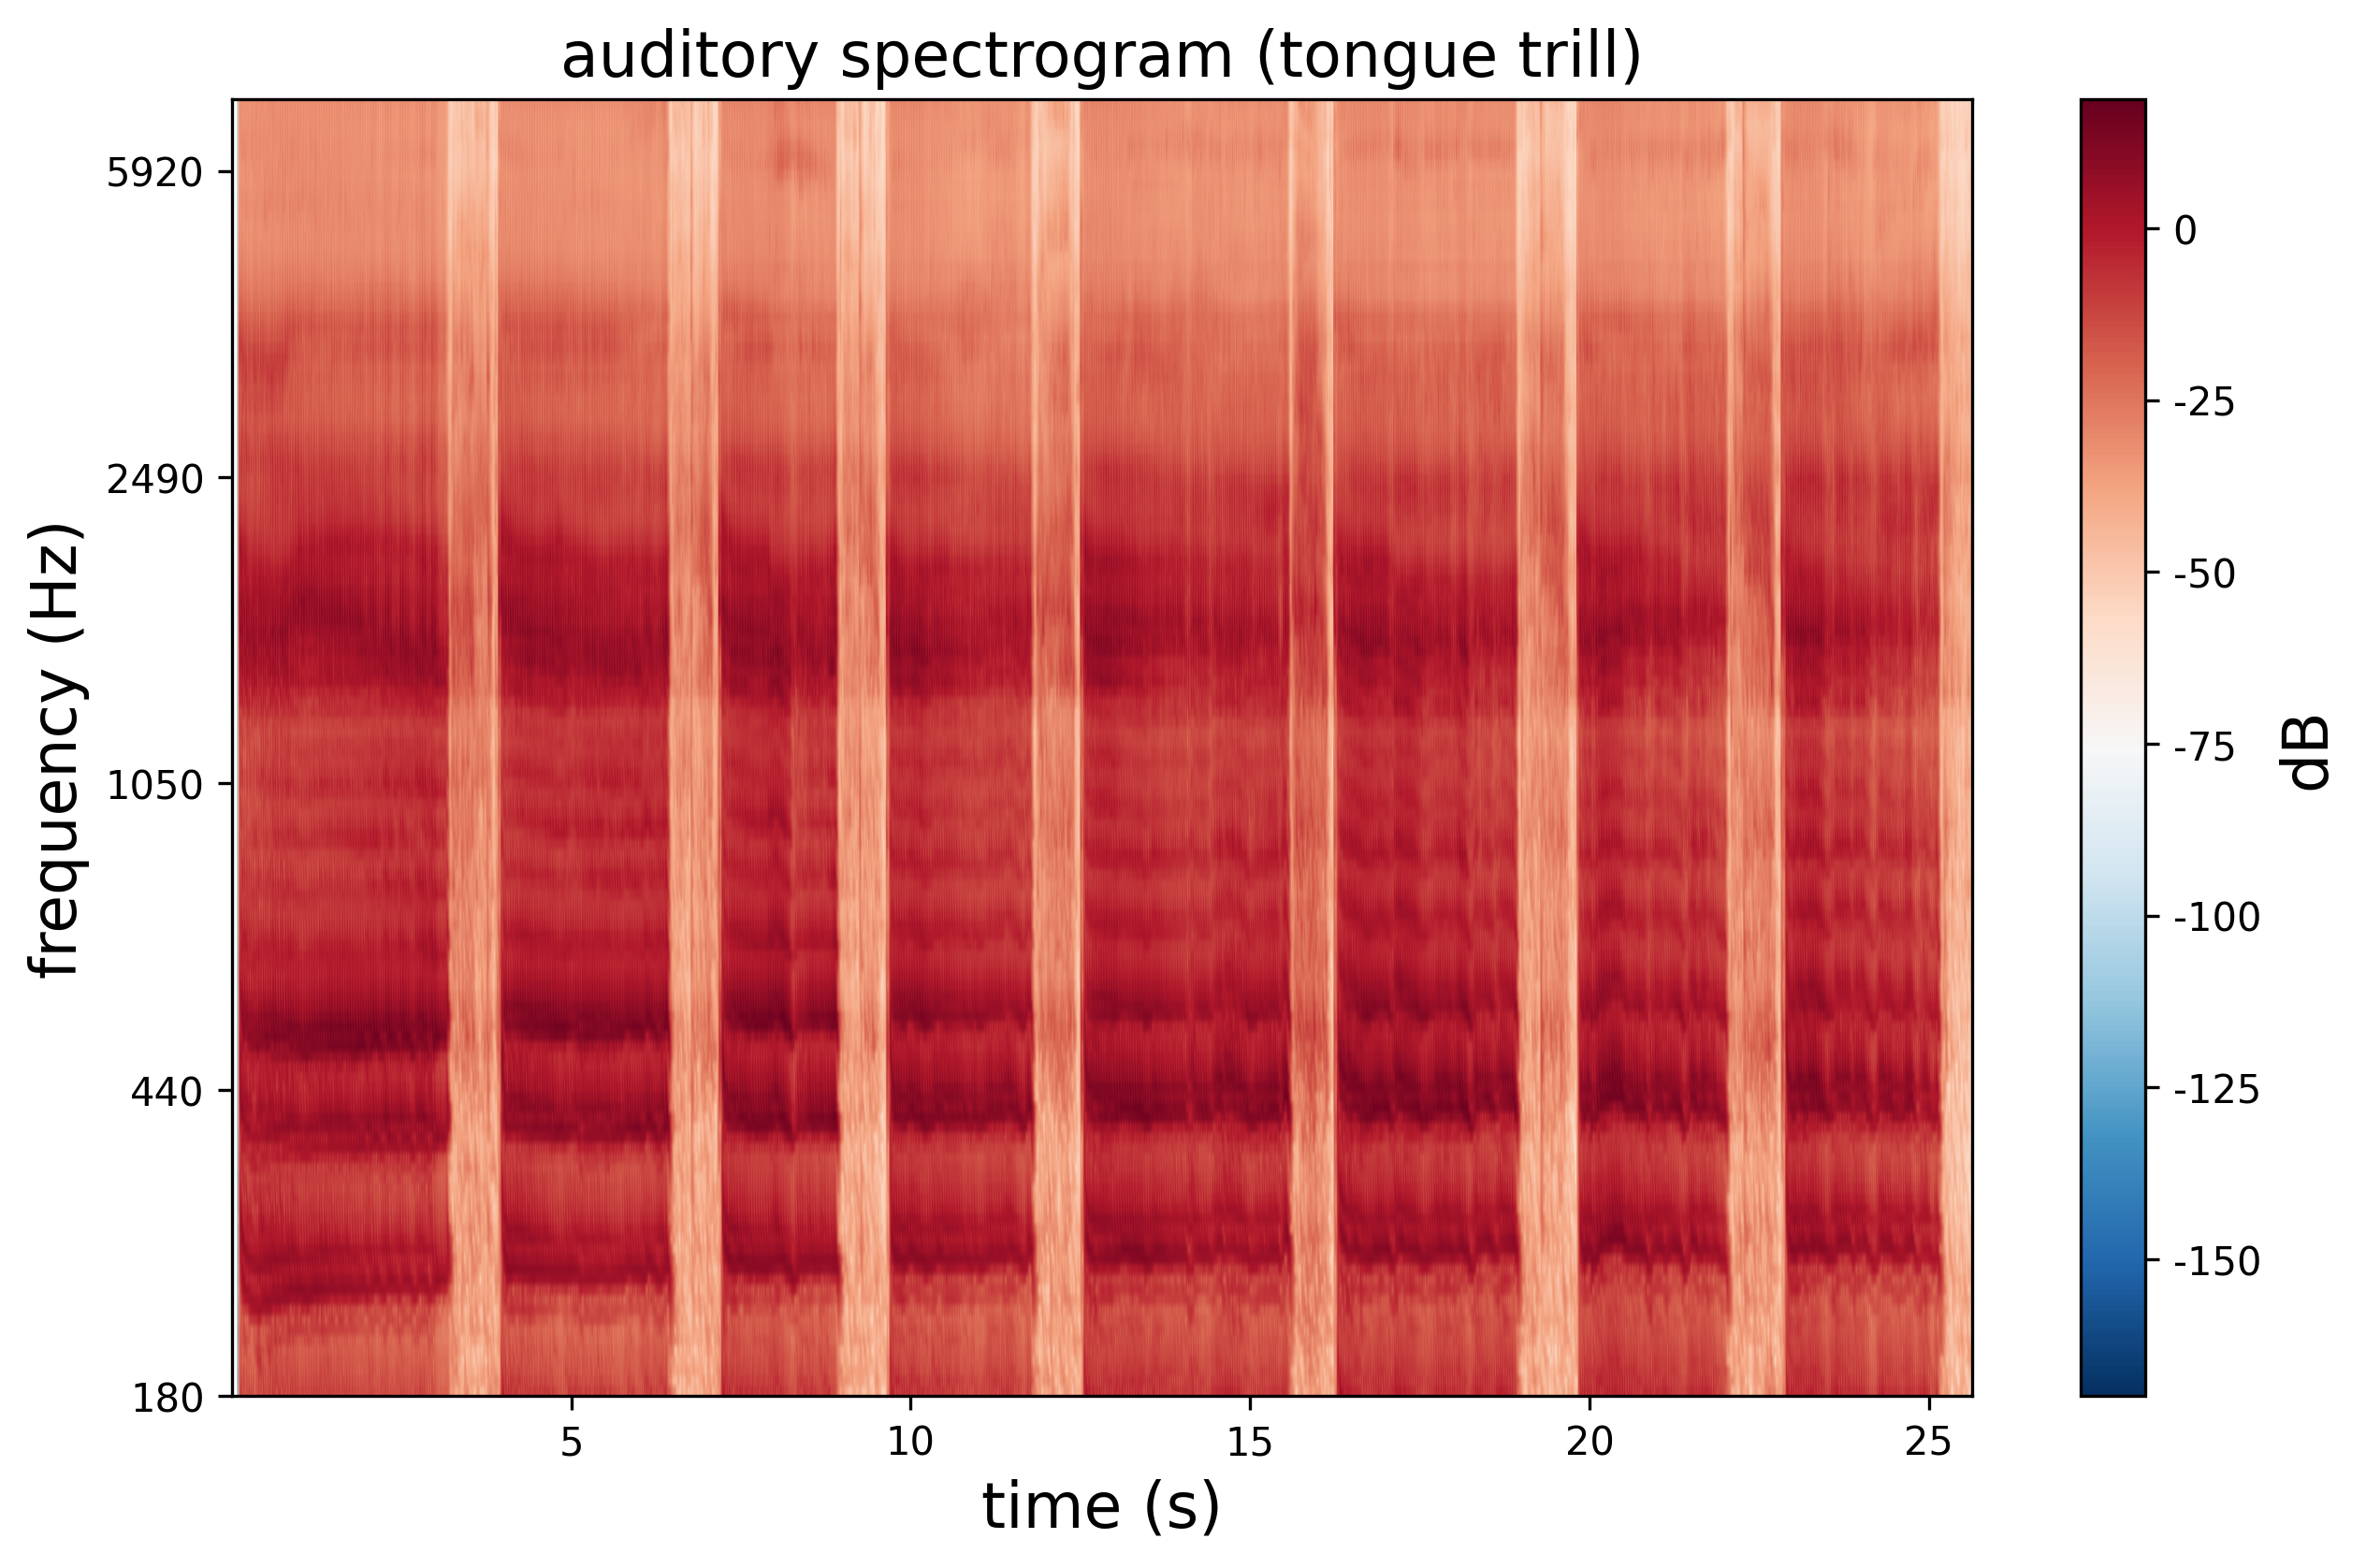
\includegraphics[width=\textwidth]{figure/tanshe.png}
%         \label{spectrogram:tanshe}
%     \end{minipage}
%     \begin{minipage}{0.49\textwidth}
%         \centering
%         \subcaption{}
%         \vspace{-0.5em}
%         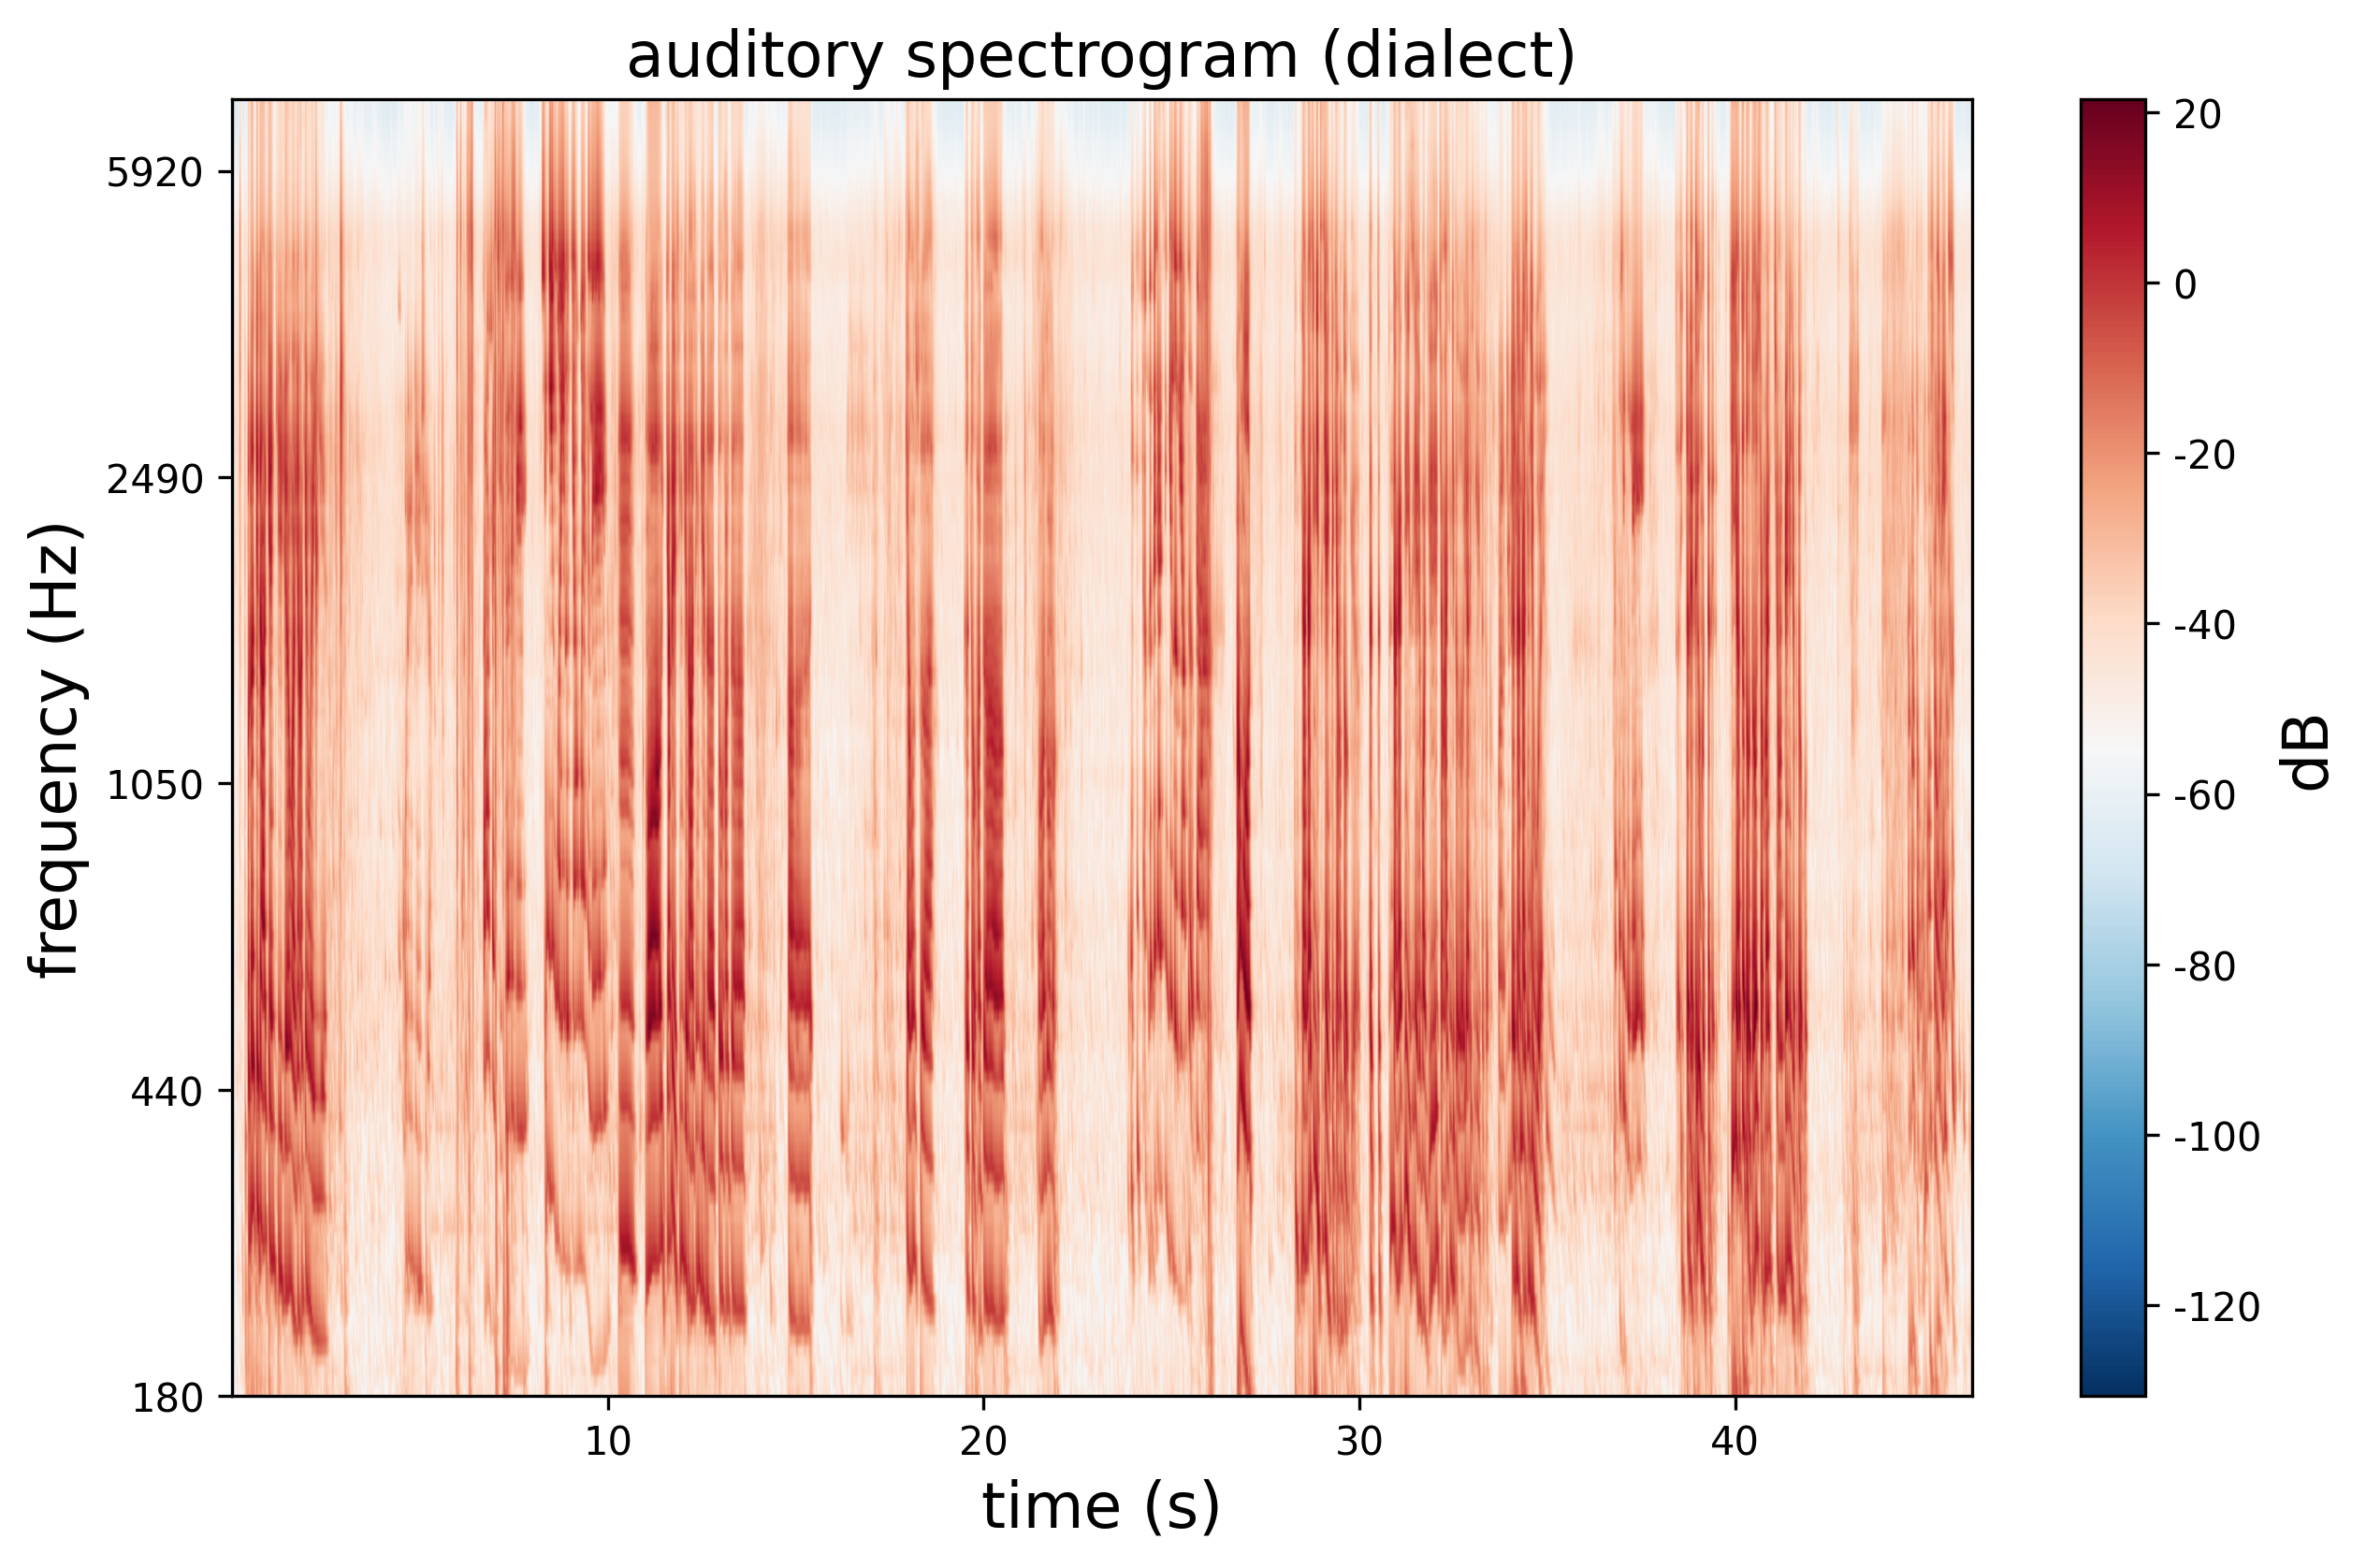
\includegraphics[width=\textwidth]{figure/dialect.png}
%         \label{spectrogram:dialect}
%     \end{minipage}
    
%     \vspace{-2em} % 调整两行子图之间的间距
    
%     % 第二行子图
%     \begin{minipage}{0.49\textwidth}
%         \centering
%         \subcaption{}
%         \vspace{-0.5em}
%         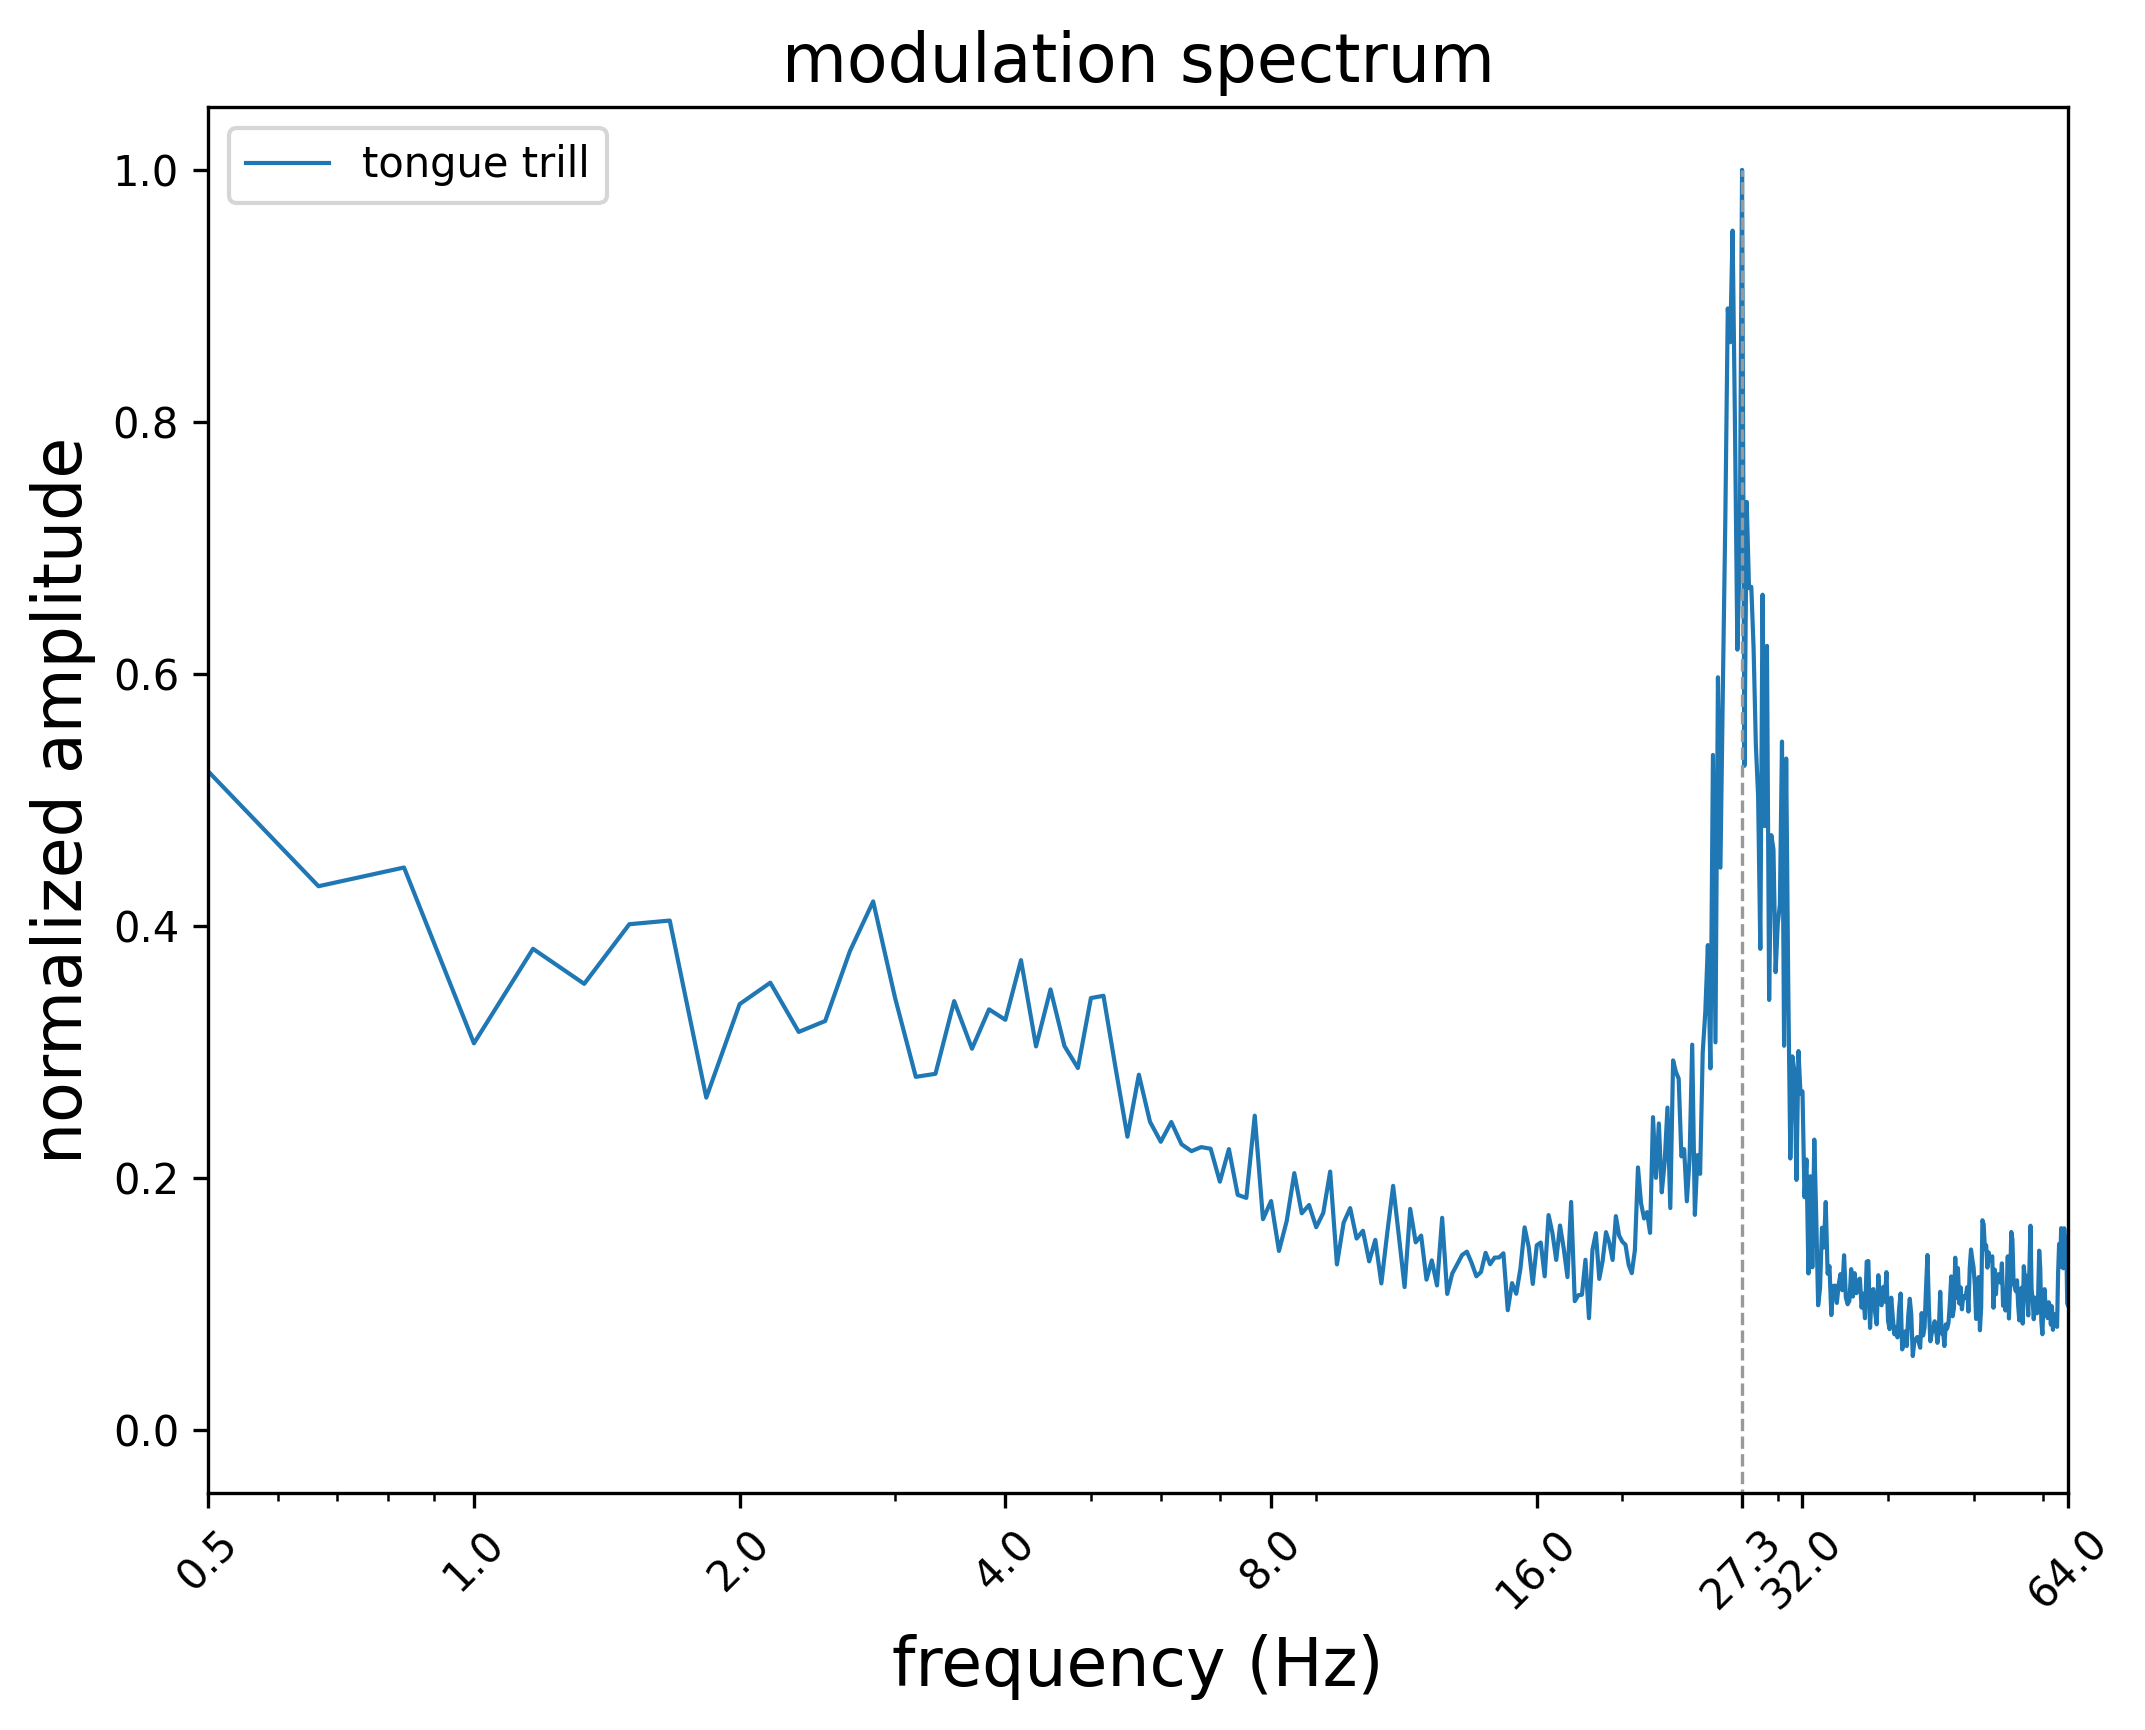
\includegraphics[width=\textwidth]{figure/spectrum_tanshe.png}
%         \label{spectrum:tanshe}
%     \end{minipage}
%     \begin{minipage}{0.49\textwidth}
%         \centering
%         \subcaption{}
%         \vspace{-0.5em}
%         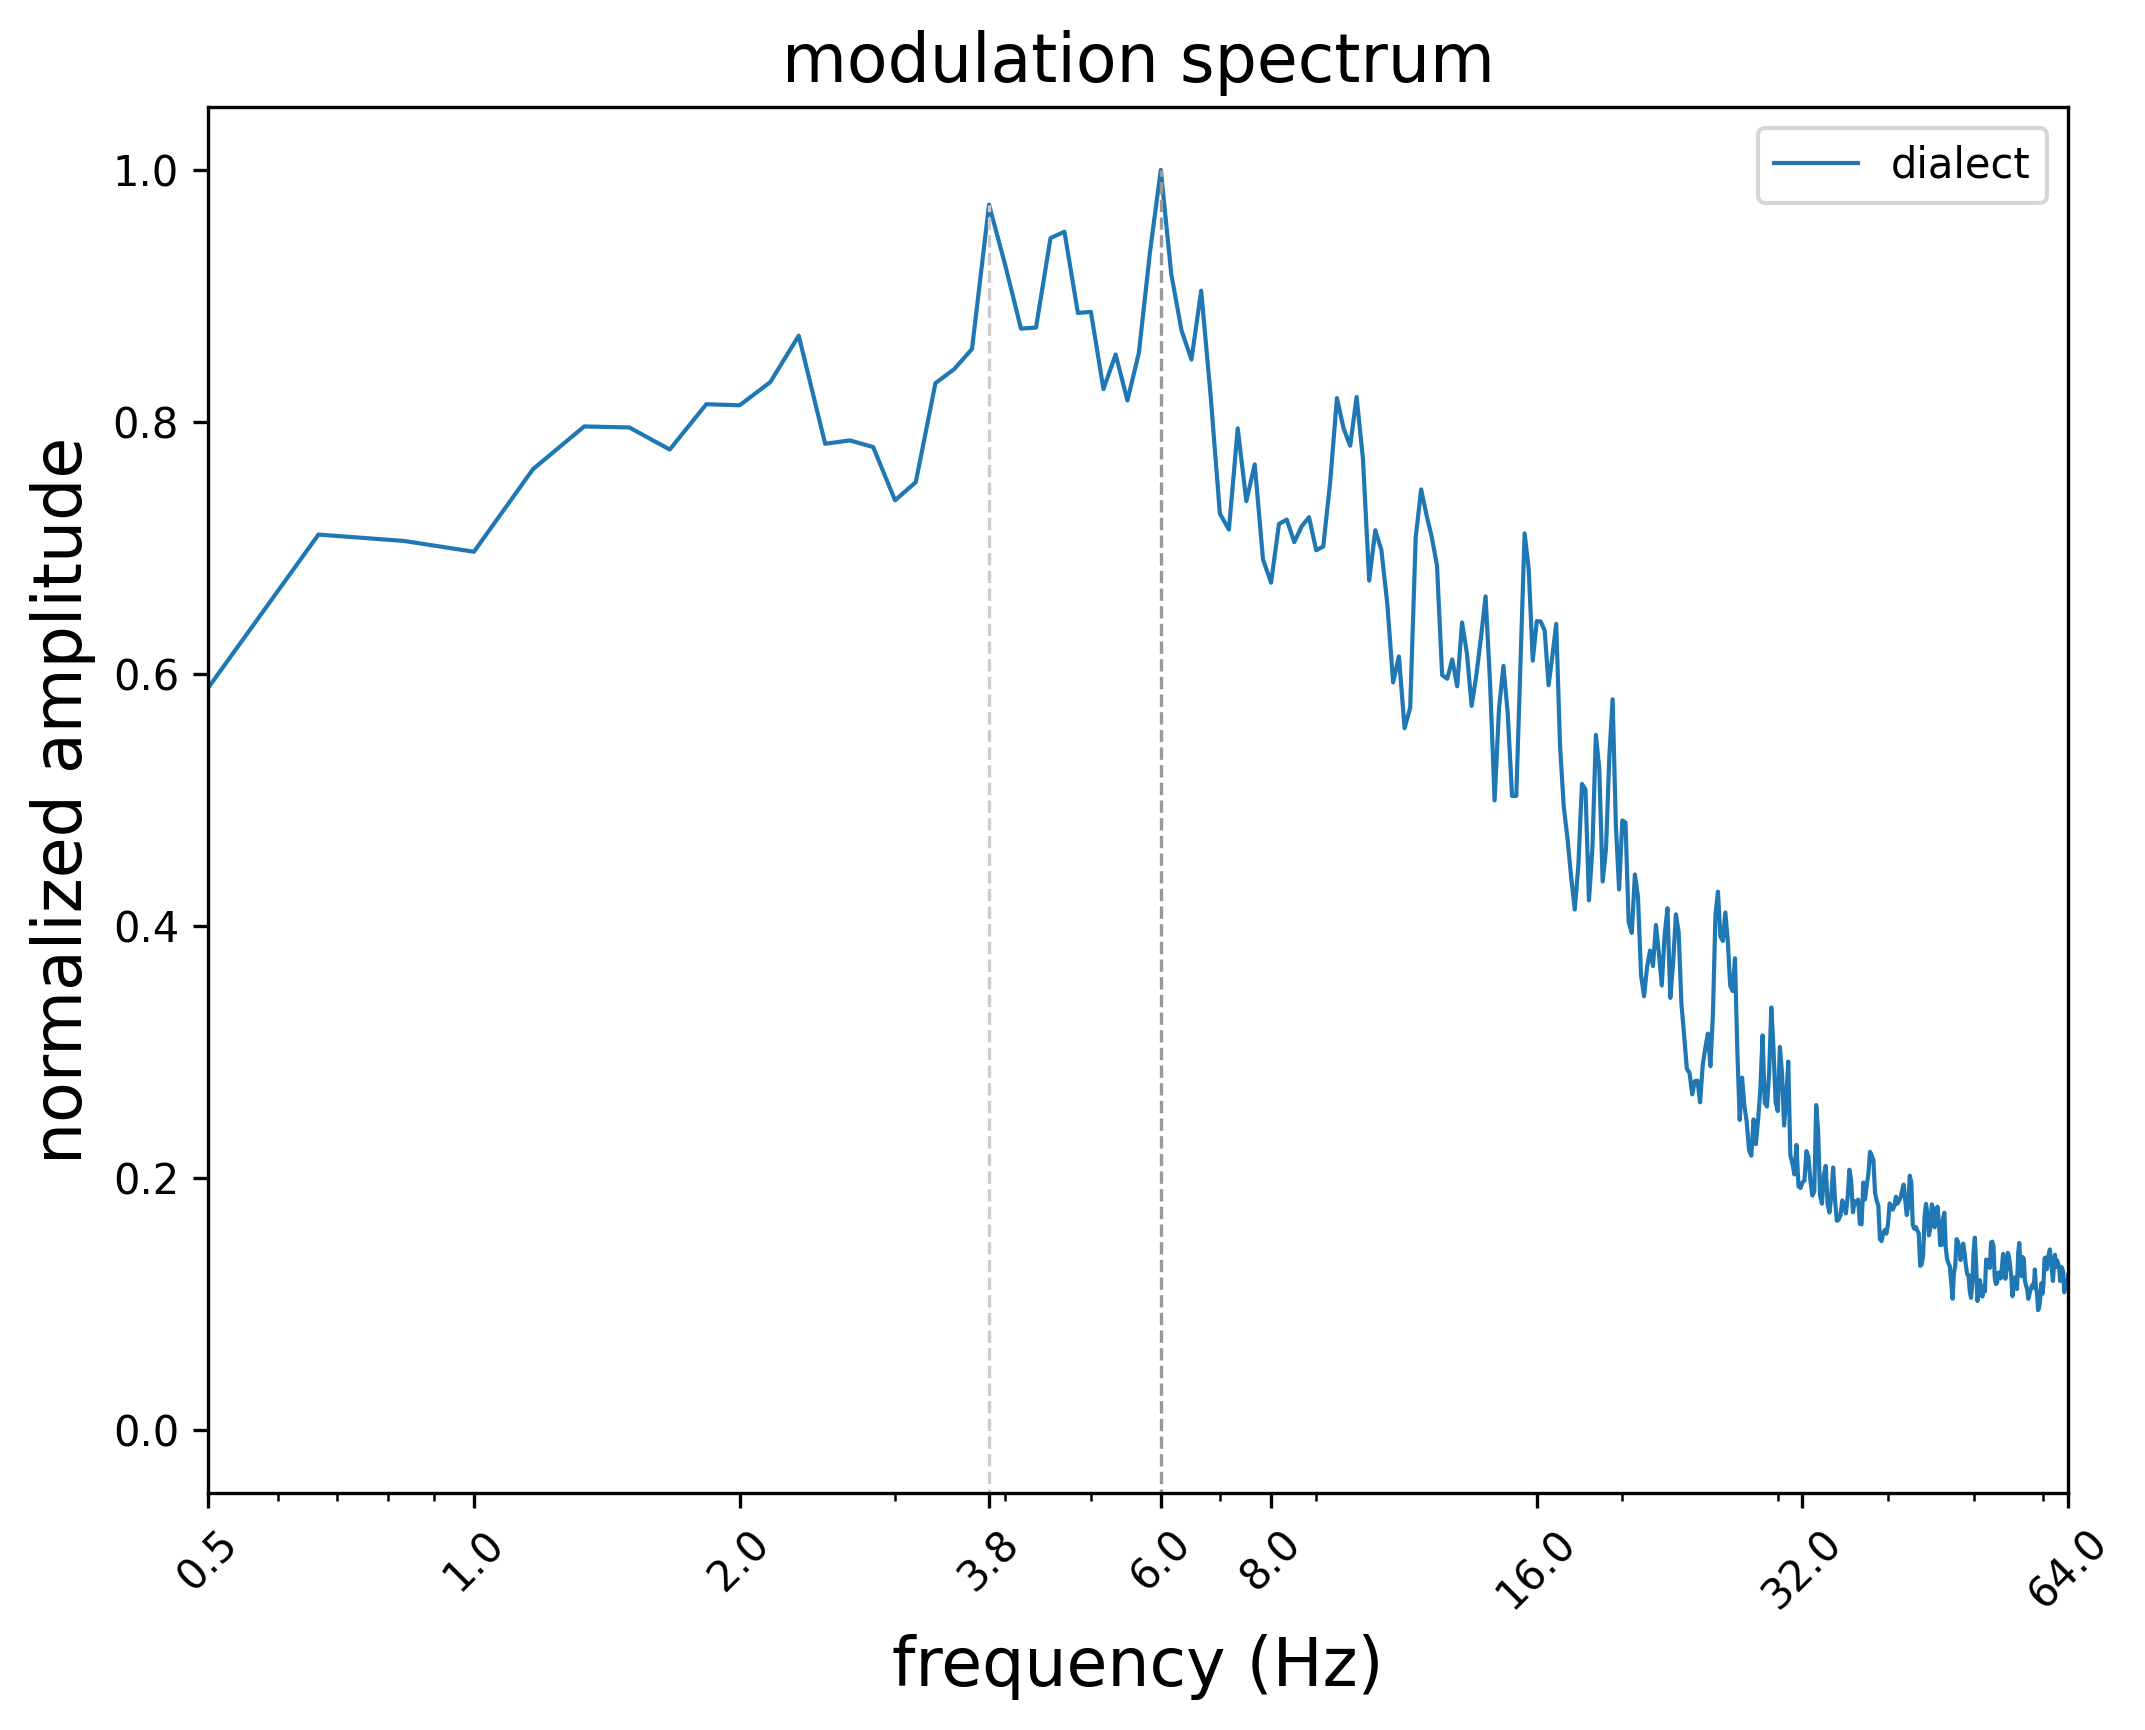
\includegraphics[width=\textwidth]{figure/spectrum_dialect.png}
%         \label{spectrum:dialect}
%     \end{minipage}
    
%     \captionsetup{labelsep=period}
%     \vspace{-1em}
%     \caption{\small 弹舌和方言交流的时频图和调制谱}
    
%     \label{fig:fig2}
% \end{figure*}


\section{讨论}

本研究旨在探讨噪音掩蔽条件下,噪音强度及滤波带宽对 1000 Hz 纯音阈值的影响。实验1的结果显示,在测试的两种噪音强度(0.64w vs 1.44w 平均功率)下,被试的纯音探测阈值并未表现出显著差异。这表明在本实验所选的强度范围内,噪音强度的变化对纯音阈值的影响不明显。实验2的结果指出,掩蔽噪音的滤波带宽对纯音阈值具有显著影响。具体而言,随着滤波器半带宽 (A) 从 100 Hz 增加到 900 Hz,纯音阈值呈现显著的线性下降趋势,即滤波器通带越宽,掩蔽效应越弱(所需信号能量越低)。

实验1未能支持\(H_1\),即未发现纯音阈值随噪音强度增大而显著升高。经典的掩蔽理论通常认为,掩蔽声强度越大,对目标声的掩蔽效应越强,阈值越高\parencite[e.g.][]{small1959pure}。本研究结果与此预期有所出入,可能的原因包括:(1) 所选的两种噪音强度差异较小,可能不足以在本实验条件下(如被试数量、实验程序敏感性)产生统计上显著的阈值差异;(2) 尽管本研究控制了设备和音量设置,实验中使用的绝对声压级也可能影响结果。需要注意的是,虽然未发现显著差异,但这并不意味着噪音没有产生掩蔽效应,只是两种强度下的掩蔽量差异不显著。

实验2的结果符合经典的听觉滤波器(或称临界带,Critical Band)理论\parencite{patterson1976auditory,fletcher1940auditory}。该理论认为,人耳在探测某一频率的纯音时,主要受到该频率附近一个特定频带(即临界带)内的噪音能量的掩蔽。在本实验中,目标纯音为 1000 Hz。当滤波器带宽较窄时(如 A=100 Hz,通带 900-1100 Hz),几乎所有噪音能量都集中在 1000 Hz 的临界带内,因此掩蔽效应最强,阈值最高。随着带宽增加(A=300 Hz,通带 700-1300 Hz;A=900 Hz,通带 100-1900 Hz),虽然总噪音功率被标准化,但越来越多的噪音能量分布在目标频率 1000 Hz 的临界带之外,这些带外噪音对 1000 Hz 纯音的掩蔽效率大大降低。因此,有效掩蔽能量减少,导致探测阈值下降。实验2的显著线性下降趋势有力地支持了听觉系统频率选择性的概念,表明被试能够有效地“滤除”或忽略与目标信号频率相距较远的噪音成分。

不过,本实验仍存在一些局限性。首先,样本量较小 (\(N\)=3),这限制了结果的普适性,也可能导致未能检测出实验1中可能存在的较小效应(统计功效不足)。其次,实验1仅测试了两个噪音强度水平,未能探索更大范围内的强度效应。第三,虽然实验中使用了标准化的设备和音量设置,但未对被试进行听力筛查以排除潜在的轻微听力损失,也未系统考虑年龄、性别等因素可能对阈值产生的影响\parencite{corso1959age,brant1990age}。第四,本研究仅使用了 1000 Hz 的纯音和高斯白噪音,结果是否能推广到其他频率、其他类型的信号(如语音)和掩蔽声,尚需进一步验证。最后,虽然滤波器参数(64阶 FIR,汉明窗)已明确,但不同滤波器设计也可能对结果产生细微影响。

\section{结\ 论}

综上所述,本研究通过心理物理学实验,考察了噪音强度和滤波带宽对 1000 Hz 纯音掩蔽阈值的影响。结果显示,在本实验条件下,噪音强度变化未引起阈值显著改变;而滤波带宽则显著影响阈值,带宽越宽,掩蔽效应越弱,阈值越低,这与听觉临界带理论的预测一致。研究结果强调了噪音频谱特性在听觉掩蔽中的关键作用。未来的研究应在更大样本、更广参数范围和更复杂听觉情境下进一步深化对噪音掩蔽机制的理解。

\printbibliography[title={\heiti 参\ 考\ 文\ 献}]

\end{document}

